\documentclass[a4paper]{book}
\usepackage{a4wide}
\usepackage{makeidx}
\usepackage{graphicx}
\usepackage{multicol}
\usepackage{float}
\usepackage{listings}
\usepackage{color}
\usepackage{textcomp}
\usepackage{alltt}
\usepackage{times}
\usepackage{ifpdf}
\ifpdf
\usepackage[pdftex,
            pagebackref=true,
            colorlinks=true,
            linkcolor=blue,
            unicode
           ]{hyperref}
\else
\usepackage[ps2pdf,
            pagebackref=true,
            colorlinks=true,
            linkcolor=blue,
            unicode
           ]{hyperref}
\usepackage{pspicture}
\fi
\usepackage[utf8]{inputenc}
\usepackage{doxygen}
\lstset{language=C++,inputencoding=utf8,basicstyle=\footnotesize,breaklines=true,breakatwhitespace=true,tabsize=8,numbers=left }
\makeindex
\setcounter{tocdepth}{3}
\renewcommand{\footrulewidth}{0.4pt}
\begin{document}
\hypersetup{pageanchor=false}
\begin{titlepage}
\vspace*{7cm}
\begin{center}
{\Large MOCLE \\[1ex]\large version2.0 }\\
\vspace*{1cm}
{\large Generated by Doxygen 1.6.1}\\
\vspace*{0.5cm}
{\small Tue Jul 27 11:21:32 2010}\\
\end{center}
\end{titlepage}
\clearemptydoublepage
\pagenumbering{roman}
\tableofcontents
\clearemptydoublepage
\pagenumbering{arabic}
\hypersetup{pageanchor=true}
\chapter{MOCLE}
\label{index}\hypertarget{index}{}\hypertarget{index_intro_sec}{}\section{Introduction}\label{index_intro_sec}
A brief introduction about MOCLE system.\hypertarget{index_install_sec}{}\section{Installation}\label{index_install_sec}
\hypertarget{index_step1}{}\subsection{Step 1: How install MOCLE}\label{index_step1}
What do to install and use MOCLE ..

\begin{DoxyAuthor}{Author}
Katti Facelli 
\end{DoxyAuthor}

\chapter{Class Index}
\section{Class Hierarchy}
This inheritance list is sorted roughly, but not completely, alphabetically:\begin{DoxyCompactList}
\item \contentsline{section}{DataSet}{\pageref{classDataSet}}{}
\item \contentsline{section}{Exception}{\pageref{classException}}{}
\item \contentsline{section}{InformationTheory}{\pageref{classInformationTheory}}{}
\begin{DoxyCompactList}
\item \contentsline{section}{NMIIndex}{\pageref{classNMIIndex}}{}
\item \contentsline{section}{VIIndex}{\pageref{classVIIndex}}{}
\end{DoxyCompactList}
\item \contentsline{section}{NnList}{\pageref{classNnList}}{}
\item \contentsline{section}{Partition}{\pageref{classPartition}}{}
\item \contentsline{section}{RelationSDN}{\pageref{classRelationSDN}}{}
\item \contentsline{section}{Similarity}{\pageref{classSimilarity}}{}
\begin{DoxyCompactList}
\item \contentsline{section}{Euclidean}{\pageref{classEuclidean}}{}
\item \contentsline{section}{Pearson}{\pageref{classPearson}}{}
\end{DoxyCompactList}
\item \contentsline{section}{SimilarityMatrix}{\pageref{classSimilarityMatrix}}{}
\item \contentsline{section}{ValidationIndex}{\pageref{classValidationIndex}}{}
\begin{DoxyCompactList}
\item \contentsline{section}{Connectivity}{\pageref{classConnectivity}}{}
\item \contentsline{section}{CRIndex}{\pageref{classCRIndex}}{}
\item \contentsline{section}{Deviation}{\pageref{classDeviation}}{}
\item \contentsline{section}{NMIIndex}{\pageref{classNMIIndex}}{}
\item \contentsline{section}{Silhouette}{\pageref{classSilhouette}}{}
\item \contentsline{section}{VIIndex}{\pageref{classVIIndex}}{}
\end{DoxyCompactList}
\end{DoxyCompactList}

\chapter{Class Index}
\section{Class List}
Here are the classes, structs, unions and interfaces with brief descriptions:\begin{DoxyCompactList}
\item\contentsline{section}{\hyperlink{classConnectivity}{Connectivity} }{\pageref{classConnectivity}}{}
\item\contentsline{section}{\hyperlink{classCRIndex}{CRIndex} }{\pageref{classCRIndex}}{}
\item\contentsline{section}{\hyperlink{classDataSet}{DataSet} (Responsible to manage the dataset file into the memory )}{\pageref{classDataSet}}{}
\item\contentsline{section}{\hyperlink{classDeviation}{Deviation} }{\pageref{classDeviation}}{}
\item\contentsline{section}{\hyperlink{classEuclidean}{Euclidean} (This class is necessary to calculate the euclidean distance )}{\pageref{classEuclidean}}{}
\item\contentsline{section}{\hyperlink{classException}{Exception} (\hyperlink{classException}{Exception} class throwed by the calculate method with one parameter of VI, NMI and CR classes )}{\pageref{classException}}{}
\item\contentsline{section}{\hyperlink{classInformationTheory}{InformationTheory} }{\pageref{classInformationTheory}}{}
\item\contentsline{section}{\hyperlink{classNMIIndex}{NMIIndex} }{\pageref{classNMIIndex}}{}
\item\contentsline{section}{\hyperlink{classNnList}{NnList} }{\pageref{classNnList}}{}
\item\contentsline{section}{\hyperlink{classPartition}{Partition} (Responsible to manage the partition file into the memory )}{\pageref{classPartition}}{}
\item\contentsline{section}{\hyperlink{classPearson}{Pearson} (Responsible to calculate the pearson correlation coefficient )}{\pageref{classPearson}}{}
\item\contentsline{section}{\hyperlink{classRelationSDN}{RelationSDN} }{\pageref{classRelationSDN}}{}
\item\contentsline{section}{\hyperlink{classSilhouette}{Silhouette} }{\pageref{classSilhouette}}{}
\item\contentsline{section}{\hyperlink{classSimilarity}{Similarity} (Responsible by management the measures of similarity )}{\pageref{classSimilarity}}{}
\item\contentsline{section}{\hyperlink{classSimilarityMatrix}{SimilarityMatrix} (Generates the matrix of similarity )}{\pageref{classSimilarityMatrix}}{}
\item\contentsline{section}{\hyperlink{classValidationIndex}{ValidationIndex} }{\pageref{classValidationIndex}}{}
\item\contentsline{section}{\hyperlink{classVIIndex}{VIIndex} }{\pageref{classVIIndex}}{}
\end{DoxyCompactList}

\chapter{Class Documentation}
\hypertarget{classConnectivity}{
\section{Connectivity Class Reference}
\label{classConnectivity}\index{Connectivity@{Connectivity}}
}


{\ttfamily \#include $<$Connectivity.h$>$}Inheritance diagram for Connectivity::\begin{figure}[H]
\begin{center}
\leavevmode
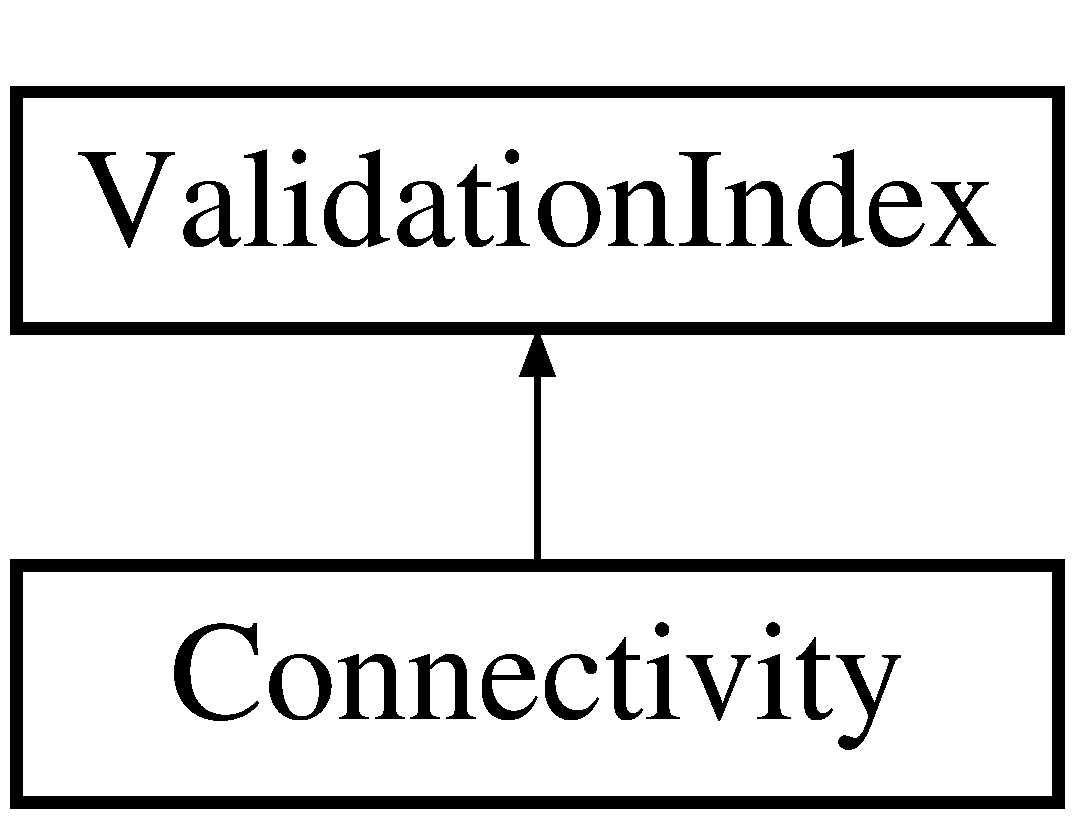
\includegraphics[height=2cm]{classConnectivity}
\end{center}
\end{figure}
\subsection*{Public Member Functions}
\begin{DoxyCompactItemize}
\item 
\hyperlink{classConnectivity_a0e8314d244056ef148ae0002cdd877a7}{Connectivity} (float aSizeNn)
\item 
virtual double \hyperlink{classConnectivity_ae132296aae336b3e3830431592611a74}{calculate} (\hyperlink{classPartition}{Partition} $\ast$pAPartition, \hyperlink{classRelationSDN}{RelationSDN} $\ast$pARelation, \hyperlink{classDataSet}{DataSet} $\ast$pDataSet)
\item 
virtual double \hyperlink{classConnectivity_a5f211e2c2ff7d5f199a985c6f6e68556}{calculate} (\hyperlink{classPartition}{Partition} \&objPartition1, \hyperlink{classPartition}{Partition} \&objPartition2)
\end{DoxyCompactItemize}


\subsection{Detailed Description}
\begin{DoxyAuthor}{Author}
Gustavo Rodrigues 
\end{DoxyAuthor}
\begin{DoxySince}{Since}
12/03/10 
\end{DoxySince}
\begin{DoxyVersion}{Version}
2.0 
\end{DoxyVersion}


Definition at line 26 of file Connectivity.h.

\subsection{Constructor \& Destructor Documentation}
\hypertarget{classConnectivity_a0e8314d244056ef148ae0002cdd877a7}{
\index{Connectivity@{Connectivity}!Connectivity@{Connectivity}}
\index{Connectivity@{Connectivity}!Connectivity@{Connectivity}}
\subsubsection[{Connectivity}]{\setlength{\rightskip}{0pt plus 5cm}Connectivity::Connectivity (float {\em aSizeNn})}}
\label{classConnectivity_a0e8314d244056ef148ae0002cdd877a7}
Does nothing 
\begin{DoxyParams}{Parameters}
\item[{\em Integer}]indicated size of nearest neighbor list \end{DoxyParams}


Definition at line 10 of file Connectivity.cpp.

\subsection{Member Function Documentation}
\hypertarget{classConnectivity_a5f211e2c2ff7d5f199a985c6f6e68556}{
\index{Connectivity@{Connectivity}!calculate@{calculate}}
\index{calculate@{calculate}!Connectivity@{Connectivity}}
\subsubsection[{calculate}]{\setlength{\rightskip}{0pt plus 5cm}double Connectivity::calculate ({\bf Partition} \& {\em objPartition1}, \/  {\bf Partition} \& {\em objPartition2})\hspace{0.3cm}{\ttfamily  \mbox{[}virtual\mbox{]}}}}
\label{classConnectivity_a5f211e2c2ff7d5f199a985c6f6e68556}
Does nothing 

Implements \hyperlink{classValidationIndex_a8b688d8d53fbdacec393730fe2bab614}{ValidationIndex}.

Definition at line 52 of file Connectivity.cpp.\hypertarget{classConnectivity_ae132296aae336b3e3830431592611a74}{
\index{Connectivity@{Connectivity}!calculate@{calculate}}
\index{calculate@{calculate}!Connectivity@{Connectivity}}
\subsubsection[{calculate}]{\setlength{\rightskip}{0pt plus 5cm}double Connectivity::calculate ({\bf Partition} $\ast$ {\em pAPartition}, \/  {\bf RelationSDN} $\ast$ {\em pARelation}, \/  {\bf DataSet} $\ast$ {\em pDataSet})\hspace{0.3cm}{\ttfamily  \mbox{[}virtual\mbox{]}}}}
\label{classConnectivity_ae132296aae336b3e3830431592611a74}
Return value of connectivity from parameter partition 
\begin{DoxyParams}{Parameters}
\item[{\em \hyperlink{classPartition}{Partition},\hyperlink{classRelationSDN}{RelationSDN}}]and \hyperlink{classDataSet}{DataSet} \end{DoxyParams}
\begin{DoxyReturn}{Returns}
Value connectivity 
\end{DoxyReturn}


Implements \hyperlink{classValidationIndex_a26fe1244f3313bd7f557149f6846fe01}{ValidationIndex}.

Definition at line 17 of file Connectivity.cpp.

References Partition::getLabelClusterOf(), NnList::getNnList(), RelationSDN::getNnList(), DataSet::getNumberOfObjects(), and DataSet::getVElements().

The documentation for this class was generated from the following files:\begin{DoxyCompactItemize}
\item 
ValidationIndex/Connectivity.h\item 
ValidationIndex/Connectivity.cpp\end{DoxyCompactItemize}

\hypertarget{classCRIndex}{
\section{CRIndex Class Reference}
\label{classCRIndex}\index{CRIndex@{CRIndex}}
}
Inheritance diagram for CRIndex::\begin{figure}[H]
\begin{center}
\leavevmode
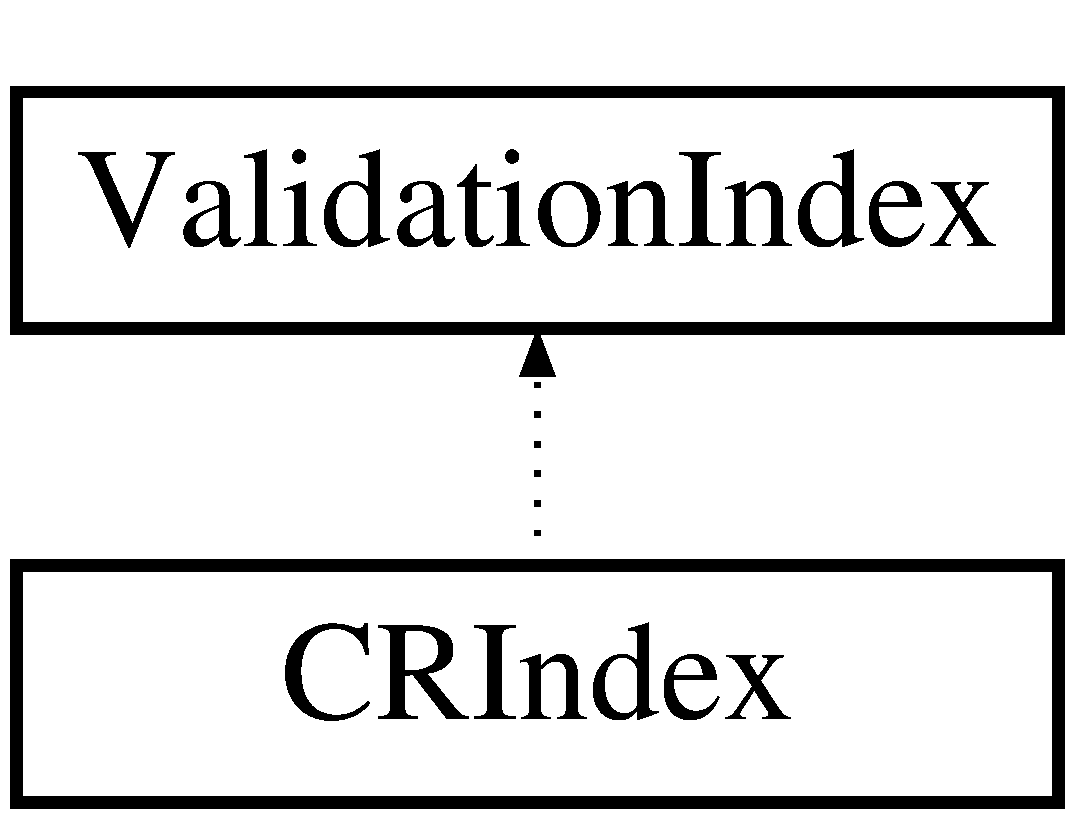
\includegraphics[height=2cm]{classCRIndex}
\end{center}
\end{figure}
\subsection*{Public Member Functions}
\begin{DoxyCompactItemize}
\item 
virtual double \hyperlink{classCRIndex_acfcf9186a522c78d67cc977aeddaf193}{calculate} (\hyperlink{classPartition}{Partition} \&objPartition1, \hyperlink{classPartition}{Partition} \&objPartition2)
\item 
virtual double \hyperlink{classCRIndex_a384b9fc6a5d271c13f7b599f17771041}{calculate} (\hyperlink{classPartition}{Partition} $\ast$pPartition, \hyperlink{classRelationSDN}{RelationSDN} $\ast$pRelation, \hyperlink{classDataSet}{DataSet} $\ast$pDataset)
\end{DoxyCompactItemize}


\subsection{Detailed Description}


Definition at line 19 of file CRIndex.h.

\subsection{Member Function Documentation}
\hypertarget{classCRIndex_a384b9fc6a5d271c13f7b599f17771041}{
\index{CRIndex@{CRIndex}!calculate@{calculate}}
\index{calculate@{calculate}!CRIndex@{CRIndex}}
\subsubsection[{calculate}]{\setlength{\rightskip}{0pt plus 5cm}double CRIndex::calculate ({\bf Partition} $\ast$ {\em pAPartition}, \/  {\bf RelationSDN} $\ast$ {\em pARelation}, \/  {\bf DataSet} $\ast$ {\em pDataSet})\hspace{0.3cm}{\ttfamily  \mbox{[}virtual\mbox{]}}}}
\label{classCRIndex_a384b9fc6a5d271c13f7b599f17771041}
Method virtual from return value of measure validation internal 
\begin{DoxyParams}{Parameters}
\item[{\em \hyperlink{classPartition}{Partition},\hyperlink{classRelationSDN}{RelationSDN}}]and \hyperlink{classDataSet}{DataSet} \end{DoxyParams}
\begin{DoxyReturn}{Returns}
Value from measure validation 
\end{DoxyReturn}


Implements \hyperlink{classValidationIndex_a26fe1244f3313bd7f557149f6846fe01}{ValidationIndex}.

Definition at line 87 of file CRIndex.cpp.\hypertarget{classCRIndex_acfcf9186a522c78d67cc977aeddaf193}{
\index{CRIndex@{CRIndex}!calculate@{calculate}}
\index{calculate@{calculate}!CRIndex@{CRIndex}}
\subsubsection[{calculate}]{\setlength{\rightskip}{0pt plus 5cm}double CRIndex::calculate ({\bf Partition} \& {\em objPartition1}, \/  {\bf Partition} \& {\em objPartition2})\hspace{0.3cm}{\ttfamily  \mbox{[}virtual\mbox{]}}}}
\label{classCRIndex_acfcf9186a522c78d67cc977aeddaf193}
Method virtual from return value of measure validation external 
\begin{DoxyParams}{Parameters}
\item[{\em \hyperlink{classPartition}{Partition}}]\end{DoxyParams}
\begin{DoxyReturn}{Returns}
Value from measure validation 
\end{DoxyReturn}


Implements \hyperlink{classValidationIndex_a8b688d8d53fbdacec393730fe2bab614}{ValidationIndex}.

Definition at line 11 of file CRIndex.cpp.

References Partition::getCluster(), Partition::getNumClusters(), and Partition::getNumObjects().

The documentation for this class was generated from the following files:\begin{DoxyCompactItemize}
\item 
ValidationIndex/CRIndex.h\item 
ValidationIndex/CRIndex.cpp\end{DoxyCompactItemize}

\hypertarget{classDataSet}{
\section{DataSet Class Reference}
\label{classDataSet}\index{DataSet@{DataSet}}
}


Responsible to manage the dataset file into the memory.  


{\ttfamily \#include $<$DataSet.h$>$}\subsection*{Public Member Functions}
\begin{DoxyCompactItemize}
\item 
\hyperlink{classDataSet_ac9b99505bafd5b1cccf8a361c3ac84a7}{DataSet} ()
\item 
\hyperlink{classDataSet_a46b0b094bd833ace0a8f69fc74fadf18}{DataSet} (string sPathADataSet, string sANameDataSet)
\item 
map$<$ string, map$<$ string, double $>$ $>$ \hyperlink{classDataSet_a17c8ba146ec31cd291ded2be3f8833d5}{generateMatrix} (\hyperlink{classSimilarity}{Similarity} $\ast$pAObSimilarity)
\item 
void \hyperlink{classDataSet_a8a5fa42fd383c845b2896fd7f3e4cce4}{tabulateMappingDataSet} ()
\item 
int \hyperlink{classDataSet_af747c49a69d26123a80a2da14eb40e13}{getNumberOfFeature} ()
\item 
int \hyperlink{classDataSet_ad871938d36c8988a8e921788cd0019f7}{getNumberOfObjects} ()
\item 
\hypertarget{classDataSet_a83456254b8ff38c9711d2b50383aa48e}{
string {\bfseries getNameDataSet} ()}
\label{classDataSet_a83456254b8ff38c9711d2b50383aa48e}

\item 
map$<$ string, vector$<$ double $>$ $>$ \hyperlink{classDataSet_ab143b593863e69f9fb13383b2917f6f5}{getMapVector} ()
\item 
\hypertarget{classDataSet_a62ad7281541ee669a1318883eb4e9aa7}{
fs::path {\bfseries getPathToDataSet} ()}
\label{classDataSet_a62ad7281541ee669a1318883eb4e9aa7}

\item 
vector$<$ string $>$ \hyperlink{classDataSet_aaa850e86d8c43a4209cc83cf5354822f}{getVElements} ()
\item 
\hyperlink{classRelationSDN}{RelationSDN} $\ast$ \hyperlink{classDataSet_a0f0dc6d4ebc1b45cce29c2bc3bbc0a75}{getRelation} (int iAPosRelation)
\item 
void \hyperlink{classDataSet_a88e3f1f9e32bd459356869c3f13401fc}{addNewRelationSDN} (\hyperlink{classSimilarity}{Similarity} $\ast$pAObSimilarity)
\item 
void \hyperlink{classDataSet_a13b30783d97d4ea7469988979afe457f}{setNameDataSet} (string sANameDataSet)
\end{DoxyCompactItemize}
\subsection*{Public Attributes}
\begin{DoxyCompactItemize}
\item 
\hypertarget{classDataSet_a4fa34425222deba63a72e973ab3b445c}{
vector$<$ \hyperlink{classSimilarity}{Similarity} $\ast$ $>$ {\bfseries vectorObSimilarity}}
\label{classDataSet_a4fa34425222deba63a72e973ab3b445c}

\end{DoxyCompactItemize}


\subsection{Detailed Description}
Responsible to manage the dataset file into the memory. \begin{DoxyAuthor}{Author}
Valter Henrique, Gustavo Henrique 
\end{DoxyAuthor}
\begin{DoxySince}{Since}
01/02/10 
\end{DoxySince}
\begin{DoxyVersion}{Version}
2.0 Dataset class is responsible to inform the data to MOCLE 
\end{DoxyVersion}


Definition at line 40 of file DataSet.h.

\subsection{Constructor \& Destructor Documentation}
\hypertarget{classDataSet_ac9b99505bafd5b1cccf8a361c3ac84a7}{
\index{DataSet@{DataSet}!DataSet@{DataSet}}
\index{DataSet@{DataSet}!DataSet@{DataSet}}
\subsubsection[{DataSet}]{\setlength{\rightskip}{0pt plus 5cm}DataSet::DataSet ()}}
\label{classDataSet_ac9b99505bafd5b1cccf8a361c3ac84a7}
Does nothing 
\begin{DoxyParams}{Parameters}
\item[{\em Don't}]have any parameter \end{DoxyParams}
\hypertarget{classDataSet_a46b0b094bd833ace0a8f69fc74fadf18}{
\index{DataSet@{DataSet}!DataSet@{DataSet}}
\index{DataSet@{DataSet}!DataSet@{DataSet}}
\subsubsection[{DataSet}]{\setlength{\rightskip}{0pt plus 5cm}DataSet::DataSet (string {\em sPathADataSet}, \/  string {\em sANameDataSet})}}
\label{classDataSet_a46b0b094bd833ace0a8f69fc74fadf18}
Ask to the user what kind format is the dataset then choose a specific method to pass the dataset to memory of the computer 
\begin{DoxyParams}{Parameters}
\item[{\em the}]path to the dataset in the computer \end{DoxyParams}


Definition at line 10 of file DataSet.cpp.

References tabulateMappingDataSet().

\subsection{Member Function Documentation}
\hypertarget{classDataSet_a88e3f1f9e32bd459356869c3f13401fc}{
\index{DataSet@{DataSet}!addNewRelationSDN@{addNewRelationSDN}}
\index{addNewRelationSDN@{addNewRelationSDN}!DataSet@{DataSet}}
\subsubsection[{addNewRelationSDN}]{\setlength{\rightskip}{0pt plus 5cm}void DataSet::addNewRelationSDN ({\bf Similarity} $\ast$ {\em pAObSimilarity})}}
\label{classDataSet_a88e3f1f9e32bd459356869c3f13401fc}
Add new object \hyperlink{classRelationSDN}{RelationSDN} in vectorRelations vector 
\begin{DoxyParams}{Parameters}
\item[{\em Object}]similarity \end{DoxyParams}
\begin{DoxyReturn}{Returns}
Don't have 
\end{DoxyReturn}


Definition at line 40 of file DataSet.cpp.

References generateMatrix(), RelationSDN::setNnList(), RelationSDN::setSimilarity(), and RelationSDN::setSimilarityMatrix().\hypertarget{classDataSet_a17c8ba146ec31cd291ded2be3f8833d5}{
\index{DataSet@{DataSet}!generateMatrix@{generateMatrix}}
\index{generateMatrix@{generateMatrix}!DataSet@{DataSet}}
\subsubsection[{generateMatrix}]{\setlength{\rightskip}{0pt plus 5cm}map$<$ string, map$<$ string, double $>$ $>$ DataSet::generateMatrix ({\bf Similarity} $\ast$ {\em pAObSimilarity})}}
\label{classDataSet_a17c8ba146ec31cd291ded2be3f8833d5}
Generate the Distance matrix get in the dataset file to the memory 
\begin{DoxyParams}{Parameters}
\item[{\em Object}]similarity \end{DoxyParams}
\begin{DoxyReturn}{Returns}
Matrix map 
\end{DoxyReturn}


Definition at line 52 of file DataSet.cpp.

References Similarity::calculate().

Referenced by addNewRelationSDN().\hypertarget{classDataSet_ab143b593863e69f9fb13383b2917f6f5}{
\index{DataSet@{DataSet}!getMapVector@{getMapVector}}
\index{getMapVector@{getMapVector}!DataSet@{DataSet}}
\subsubsection[{getMapVector}]{\setlength{\rightskip}{0pt plus 5cm}map$<$ string, vector$<$ double $>$ $>$ DataSet::getMapVector ()}}
\label{classDataSet_ab143b593863e69f9fb13383b2917f6f5}
Returns the dataset mapped int th struct \begin{DoxyReturn}{Returns}
pathToDataSet 
\end{DoxyReturn}


Definition at line 131 of file DataSet.cpp.

Referenced by Silhouette::calculate(), and Deviation::calculate().\hypertarget{classDataSet_af747c49a69d26123a80a2da14eb40e13}{
\index{DataSet@{DataSet}!getNumberOfFeature@{getNumberOfFeature}}
\index{getNumberOfFeature@{getNumberOfFeature}!DataSet@{DataSet}}
\subsubsection[{getNumberOfFeature}]{\setlength{\rightskip}{0pt plus 5cm}int DataSet::getNumberOfFeature ()}}
\label{classDataSet_af747c49a69d26123a80a2da14eb40e13}
Returns the number of features existing in dataset \begin{DoxyReturn}{Returns}
iNumFeatures 
\end{DoxyReturn}


Definition at line 119 of file DataSet.cpp.\hypertarget{classDataSet_ad871938d36c8988a8e921788cd0019f7}{
\index{DataSet@{DataSet}!getNumberOfObjects@{getNumberOfObjects}}
\index{getNumberOfObjects@{getNumberOfObjects}!DataSet@{DataSet}}
\subsubsection[{getNumberOfObjects}]{\setlength{\rightskip}{0pt plus 5cm}int DataSet::getNumberOfObjects ()}}
\label{classDataSet_ad871938d36c8988a8e921788cd0019f7}
Returns the number of objects existing in dataset \begin{DoxyReturn}{Returns}
iNumFeatures 
\end{DoxyReturn}


Definition at line 123 of file DataSet.cpp.

Referenced by Connectivity::calculate(), and Partition::generateRandomPartition().\hypertarget{classDataSet_a0f0dc6d4ebc1b45cce29c2bc3bbc0a75}{
\index{DataSet@{DataSet}!getRelation@{getRelation}}
\index{getRelation@{getRelation}!DataSet@{DataSet}}
\subsubsection[{getRelation}]{\setlength{\rightskip}{0pt plus 5cm}{\bf RelationSDN} $\ast$ DataSet::getRelation (int {\em iAPosRelation})}}
\label{classDataSet_a0f0dc6d4ebc1b45cce29c2bc3bbc0a75}
Return pointer for vector \hyperlink{classRelationSDN}{RelationSDN} 
\begin{DoxyParams}{Parameters}
\item[{\em Position}]of vector \end{DoxyParams}
\begin{DoxyReturn}{Returns}
RelationSDN$\ast$ 
\end{DoxyReturn}


Definition at line 36 of file DataSet.cpp.\hypertarget{classDataSet_aaa850e86d8c43a4209cc83cf5354822f}{
\index{DataSet@{DataSet}!getVElements@{getVElements}}
\index{getVElements@{getVElements}!DataSet@{DataSet}}
\subsubsection[{getVElements}]{\setlength{\rightskip}{0pt plus 5cm}vector$<$ string $>$ DataSet::getVElements ()}}
\label{classDataSet_aaa850e86d8c43a4209cc83cf5354822f}
Return vector of all objects from dataset 
\begin{DoxyParams}{Parameters}
\item[{\em Don't}]have \end{DoxyParams}
\begin{DoxyReturn}{Returns}
vector$<$string$>$ 
\end{DoxyReturn}


Definition at line 32 of file DataSet.cpp.

Referenced by Connectivity::calculate().\hypertarget{classDataSet_a13b30783d97d4ea7469988979afe457f}{
\index{DataSet@{DataSet}!setNameDataSet@{setNameDataSet}}
\index{setNameDataSet@{setNameDataSet}!DataSet@{DataSet}}
\subsubsection[{setNameDataSet}]{\setlength{\rightskip}{0pt plus 5cm}void DataSet::setNameDataSet (string {\em sANameDataSet})}}
\label{classDataSet_a13b30783d97d4ea7469988979afe457f}
Set the name of the dataset file 
\begin{DoxyParams}{Parameters}
\item[{\em String}]sANameDataset \end{DoxyParams}
\begin{DoxyReturn}{Returns}
Don't have 
\end{DoxyReturn}


Definition at line 135 of file DataSet.cpp.\hypertarget{classDataSet_a8a5fa42fd383c845b2896fd7f3e4cce4}{
\index{DataSet@{DataSet}!tabulateMappingDataSet@{tabulateMappingDataSet}}
\index{tabulateMappingDataSet@{tabulateMappingDataSet}!DataSet@{DataSet}}
\subsubsection[{tabulateMappingDataSet}]{\setlength{\rightskip}{0pt plus 5cm}void DataSet::tabulateMappingDataSet ()}}
\label{classDataSet_a8a5fa42fd383c845b2896fd7f3e4cce4}
Read the file passed in the argument pathADatSet and allocate in the memory 
\begin{DoxyParams}{Parameters}
\item[{\em pathADataSet}]receive the path from the dataset \end{DoxyParams}


Definition at line 77 of file DataSet.cpp.

Referenced by DataSet().

The documentation for this class was generated from the following files:\begin{DoxyCompactItemize}
\item 
DataSet.h\item 
DataSet.cpp\end{DoxyCompactItemize}

\hypertarget{classDeviation}{
\section{Deviation Class Reference}
\label{classDeviation}\index{Deviation@{Deviation}}
}


{\ttfamily \#include $<$Deviation.h$>$}Inheritance diagram for Deviation::\begin{figure}[H]
\begin{center}
\leavevmode
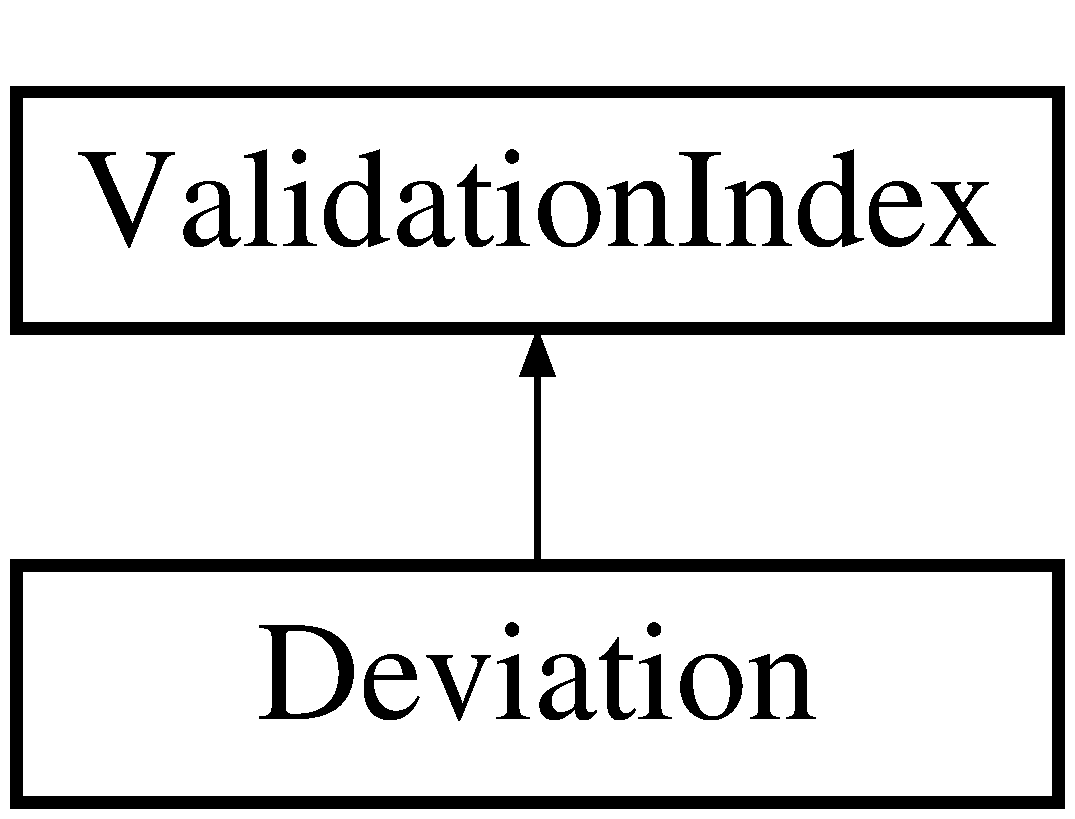
\includegraphics[height=2cm]{classDeviation}
\end{center}
\end{figure}
\subsection*{Public Member Functions}
\begin{DoxyCompactItemize}
\item 
\hyperlink{classDeviation_ac6a194e1389f1b31ab8b80b80cb6e74e}{Deviation} ()
\item 
virtual double \hyperlink{classDeviation_aefedb81474f0d06827a2ceaecd93f43c}{calculate} (\hyperlink{classPartition}{Partition} $\ast$pAPartition, \hyperlink{classRelationSDN}{RelationSDN} $\ast$pARelation, \hyperlink{classDataSet}{DataSet} $\ast$pDataSet)
\item 
virtual double \hyperlink{classDeviation_af722cf601ea21cc689a77c1de470bcb5}{calculate} (\hyperlink{classPartition}{Partition} \&objPartition1, \hyperlink{classPartition}{Partition} \&objPartition2)
\end{DoxyCompactItemize}


\subsection{Detailed Description}
\begin{DoxyAuthor}{Author}
Gustavo Rodrigues 
\end{DoxyAuthor}
\begin{DoxySince}{Since}
12/03/10 
\end{DoxySince}
\begin{DoxyVersion}{Version}
2.0 
\end{DoxyVersion}


Definition at line 25 of file Deviation.h.

\subsection{Constructor \& Destructor Documentation}
\hypertarget{classDeviation_ac6a194e1389f1b31ab8b80b80cb6e74e}{
\index{Deviation@{Deviation}!Deviation@{Deviation}}
\index{Deviation@{Deviation}!Deviation@{Deviation}}
\subsubsection[{Deviation}]{\setlength{\rightskip}{0pt plus 5cm}Deviation::Deviation ()}}
\label{classDeviation_ac6a194e1389f1b31ab8b80b80cb6e74e}
Does nothing 
\begin{DoxyParams}{Parameters}
\item[{\em Don't}]have any parameter \end{DoxyParams}


Definition at line 11 of file Deviation.cpp.

\subsection{Member Function Documentation}
\hypertarget{classDeviation_af722cf601ea21cc689a77c1de470bcb5}{
\index{Deviation@{Deviation}!calculate@{calculate}}
\index{calculate@{calculate}!Deviation@{Deviation}}
\subsubsection[{calculate}]{\setlength{\rightskip}{0pt plus 5cm}double Deviation::calculate ({\bf Partition} \& {\em objPartition1}, \/  {\bf Partition} \& {\em objPartition2})\hspace{0.3cm}{\ttfamily  \mbox{[}virtual\mbox{]}}}}
\label{classDeviation_af722cf601ea21cc689a77c1de470bcb5}
Does nothing 

Implements \hyperlink{classValidationIndex_a8b688d8d53fbdacec393730fe2bab614}{ValidationIndex}.

Definition at line 40 of file Deviation.cpp.\hypertarget{classDeviation_aefedb81474f0d06827a2ceaecd93f43c}{
\index{Deviation@{Deviation}!calculate@{calculate}}
\index{calculate@{calculate}!Deviation@{Deviation}}
\subsubsection[{calculate}]{\setlength{\rightskip}{0pt plus 5cm}double Deviation::calculate ({\bf Partition} $\ast$ {\em pAPartition}, \/  {\bf RelationSDN} $\ast$ {\em pARelation}, \/  {\bf DataSet} $\ast$ {\em pDataSet})\hspace{0.3cm}{\ttfamily  \mbox{[}virtual\mbox{]}}}}
\label{classDeviation_aefedb81474f0d06827a2ceaecd93f43c}
Return value of deviation from parameter partition 
\begin{DoxyParams}{Parameters}
\item[{\em \hyperlink{classPartition}{Partition},\hyperlink{classRelationSDN}{RelationSDN}}]and \hyperlink{classDataSet}{DataSet} \end{DoxyParams}
\begin{DoxyReturn}{Returns}
Value deviation 
\end{DoxyReturn}


calculate the summed distances for each pattern of a cluster 

Implements \hyperlink{classValidationIndex_a26fe1244f3313bd7f557149f6846fe01}{ValidationIndex}.

Definition at line 15 of file Deviation.cpp.

References Similarity::calculate(), Partition::getCentroidInCluster(), DataSet::getMapVector(), Partition::getObjectsInCluster(), RelationSDN::getSimilarity(), and Partition::getVectorObjCluster().

The documentation for this class was generated from the following files:\begin{DoxyCompactItemize}
\item 
ValidationIndex/Deviation.h\item 
ValidationIndex/Deviation.cpp\end{DoxyCompactItemize}

\hypertarget{classEuclidean}{
\section{Euclidean Class Reference}
\label{classEuclidean}\index{Euclidean@{Euclidean}}
}


This class is necessary to calculate the euclidean distance.  


{\ttfamily \#include $<$Euclidean.h$>$}Inheritance diagram for Euclidean::\begin{figure}[H]
\begin{center}
\leavevmode
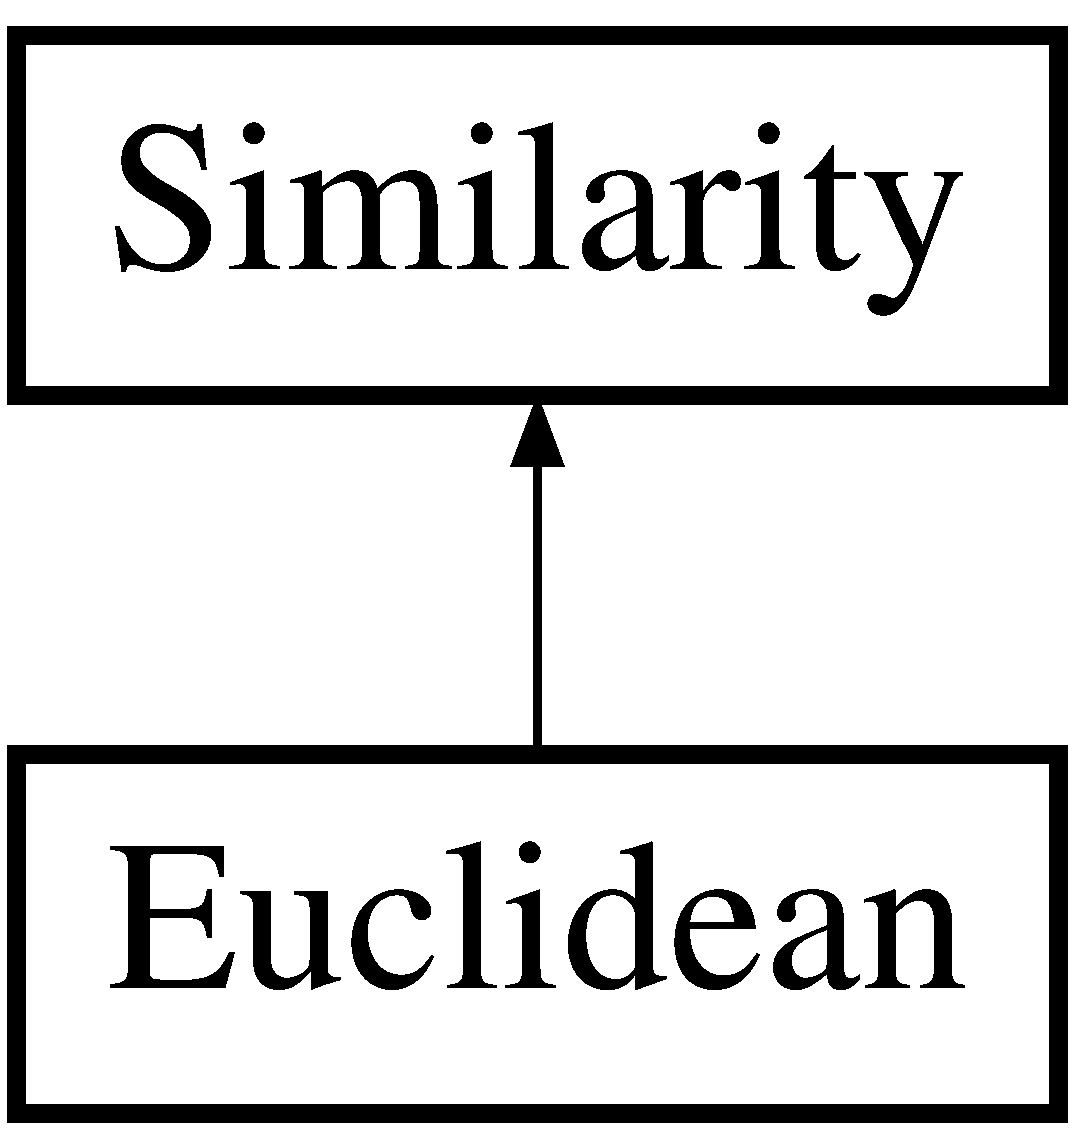
\includegraphics[height=2cm]{classEuclidean}
\end{center}
\end{figure}
\subsection*{Public Member Functions}
\begin{DoxyCompactItemize}
\item 
double \hyperlink{classEuclidean_a732c1c959cc6978d4e9050bc42fda186}{calculate} (const vector$<$ double $>$ \&vectorAPattern\_\-1, const vector$<$ double $>$ \&vectorAPattern\_\-2)
\end{DoxyCompactItemize}


\subsection{Detailed Description}
This class is necessary to calculate the euclidean distance. \begin{DoxyAuthor}{Author}
Valter Henrique 
\end{DoxyAuthor}
\begin{DoxySince}{Since}
27/02/10 
\end{DoxySince}
\begin{DoxyVersion}{Version}
2.0 This class is necessary to calculate the euclidean distance, this is made by method calculate 
\end{DoxyVersion}


Definition at line 21 of file Euclidean.h.

\subsection{Member Function Documentation}
\hypertarget{classEuclidean_a732c1c959cc6978d4e9050bc42fda186}{
\index{Euclidean@{Euclidean}!calculate@{calculate}}
\index{calculate@{calculate}!Euclidean@{Euclidean}}
\subsubsection[{calculate}]{\setlength{\rightskip}{0pt plus 5cm}double Euclidean::calculate (const vector$<$ double $>$ \& {\em vectorAPattern\_\-1}, \/  const vector$<$ double $>$ \& {\em vectorAPattern\_\-2})\hspace{0.3cm}{\ttfamily  \mbox{[}virtual\mbox{]}}}}
\label{classEuclidean_a732c1c959cc6978d4e9050bc42fda186}
Calculate the distance euclidean \begin{DoxyReturn}{Returns}
the distance euclidean beween the dois pattern passed to the method 
\end{DoxyReturn}


Implements \hyperlink{classSimilarity_a3ff3d3622d8a45b15531bc143308b2ae}{Similarity}.

Definition at line 15 of file Euclidean.cpp.

The documentation for this class was generated from the following files:\begin{DoxyCompactItemize}
\item 
Euclidean.h\item 
Euclidean.cpp\end{DoxyCompactItemize}

\hypertarget{classException}{
\section{Exception Class Reference}
\label{classException}\index{Exception@{Exception}}
}


\hyperlink{classException}{Exception} class throwed by the calculate method with one parameter of VI, NMI and CR classes.  


{\ttfamily \#include $<$Exception.h$>$}\subsection*{Public Member Functions}
\begin{DoxyCompactItemize}
\item 
\hyperlink{classException_a1b78336bb26edf8e784783cc150c5801}{Exception} ()
\item 
void \hyperlink{classException_aca2f9cfcfdfede80fc028a4150f0af48}{showError} ()
\end{DoxyCompactItemize}


\subsection{Detailed Description}
\hyperlink{classException}{Exception} class throwed by the calculate method with one parameter of VI, NMI and CR classes. \begin{DoxyAuthor}{Author}
Vinicius Lopes 
\end{DoxyAuthor}
\begin{DoxySince}{Since}
27/02/10 
\end{DoxySince}
\begin{DoxyVersion}{Version}
1.0 All the exception that occured in MOCLE is gonna be treated in this class 
\end{DoxyVersion}


Definition at line 23 of file Exception.h.

\subsection{Constructor \& Destructor Documentation}
\hypertarget{classException_a1b78336bb26edf8e784783cc150c5801}{
\index{Exception@{Exception}!Exception@{Exception}}
\index{Exception@{Exception}!Exception@{Exception}}
\subsubsection[{Exception}]{\setlength{\rightskip}{0pt plus 5cm}Exception::Exception ()}}
\label{classException_a1b78336bb26edf8e784783cc150c5801}
Does nothing 

Definition at line 13 of file Exception.cpp.

\subsection{Member Function Documentation}
\hypertarget{classException_aca2f9cfcfdfede80fc028a4150f0af48}{
\index{Exception@{Exception}!showError@{showError}}
\index{showError@{showError}!Exception@{Exception}}
\subsubsection[{showError}]{\setlength{\rightskip}{0pt plus 5cm}void Exception::showError ()}}
\label{classException_aca2f9cfcfdfede80fc028a4150f0af48}
Calculate the distance euclidean \begin{DoxyReturn}{Returns}
the distance euclidean beween the dois pattern passed to the method 
\end{DoxyReturn}


Definition at line 15 of file Exception.cpp.

The documentation for this class was generated from the following files:\begin{DoxyCompactItemize}
\item 
Exception.h\item 
Exception.cpp\end{DoxyCompactItemize}

\hypertarget{classInformationTheory}{
\section{InformationTheory Class Reference}
\label{classInformationTheory}\index{InformationTheory@{InformationTheory}}
}


{\ttfamily \#include $<$InformationTheory.h$>$}Inheritance diagram for InformationTheory::\begin{figure}[H]
\begin{center}
\leavevmode
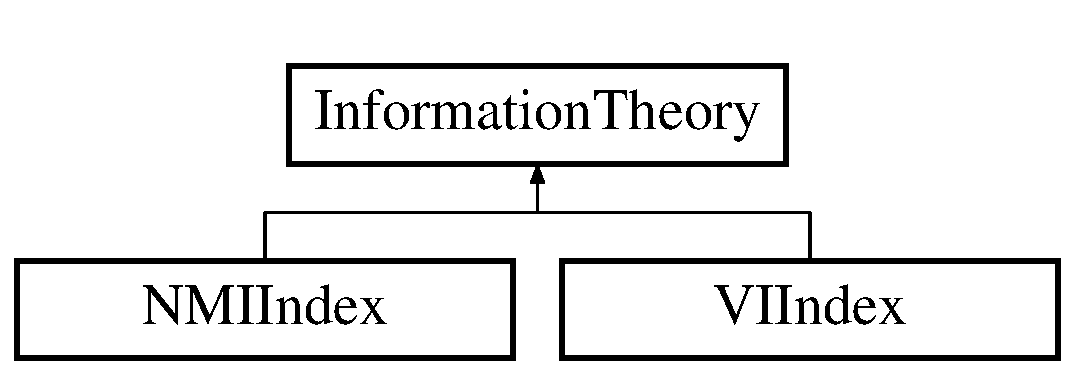
\includegraphics[height=2cm]{classInformationTheory}
\end{center}
\end{figure}
\subsection*{Protected Member Functions}
\begin{DoxyCompactItemize}
\item 
\hypertarget{classInformationTheory_ab9f75d2afd8a139f17f09c4e5ceb1019}{
double {\bfseries enthropy} (\hyperlink{classPartition}{Partition} \&objPartition)}
\label{classInformationTheory_ab9f75d2afd8a139f17f09c4e5ceb1019}

\item 
\hypertarget{classInformationTheory_a169e8d286d0b4333dfce9e54d1dcd703}{
double {\bfseries mutualInformation} (\hyperlink{classPartition}{Partition} \&objPartition1, \hyperlink{classPartition}{Partition} \&objPartition2)}
\label{classInformationTheory_a169e8d286d0b4333dfce9e54d1dcd703}

\end{DoxyCompactItemize}


\subsection{Detailed Description}
\begin{DoxyAuthor}{Author}
Vinicius 
\end{DoxyAuthor}
\begin{DoxySince}{Since}
??/$\backslash$?? 
\end{DoxySince}
\begin{DoxyVersion}{Version}
2.0 
\end{DoxyVersion}


Definition at line 16 of file InformationTheory.h.

The documentation for this class was generated from the following files:\begin{DoxyCompactItemize}
\item 
InformationTheory.h\item 
InformationTheory.cpp\end{DoxyCompactItemize}

\hypertarget{classNMIIndex}{
\section{NMIIndex Class Reference}
\label{classNMIIndex}\index{NMIIndex@{NMIIndex}}
}
Inheritance diagram for NMIIndex::\begin{figure}[H]
\begin{center}
\leavevmode
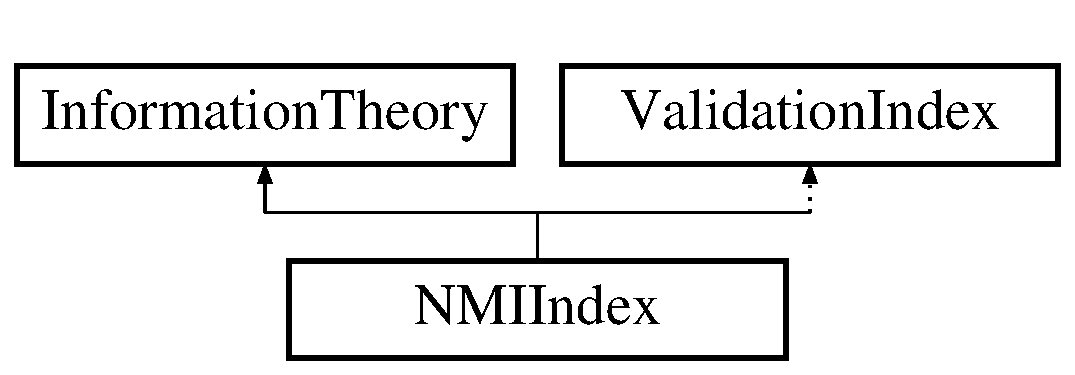
\includegraphics[height=2cm]{classNMIIndex}
\end{center}
\end{figure}
\subsection*{Public Member Functions}
\begin{DoxyCompactItemize}
\item 
virtual double \hyperlink{classNMIIndex_a3d2c254720bd825119d1cd7905daa50f}{calculate} (\hyperlink{classPartition}{Partition} \&objPartition1, \hyperlink{classPartition}{Partition} \&objPartition2)
\item 
virtual double \hyperlink{classNMIIndex_a930fb32a05cbba0f427510536c204694}{calculate} (\hyperlink{classPartition}{Partition} $\ast$pPartition, \hyperlink{classRelationSDN}{RelationSDN} $\ast$pRelation, \hyperlink{classDataSet}{DataSet} $\ast$pDataset)
\end{DoxyCompactItemize}


\subsection{Detailed Description}


Definition at line 19 of file NMIIndex.h.

\subsection{Member Function Documentation}
\hypertarget{classNMIIndex_a930fb32a05cbba0f427510536c204694}{
\index{NMIIndex@{NMIIndex}!calculate@{calculate}}
\index{calculate@{calculate}!NMIIndex@{NMIIndex}}
\subsubsection[{calculate}]{\setlength{\rightskip}{0pt plus 5cm}double NMIIndex::calculate ({\bf Partition} $\ast$ {\em pAPartition}, \/  {\bf RelationSDN} $\ast$ {\em pARelation}, \/  {\bf DataSet} $\ast$ {\em pDataSet})\hspace{0.3cm}{\ttfamily  \mbox{[}virtual\mbox{]}}}}
\label{classNMIIndex_a930fb32a05cbba0f427510536c204694}
Method virtual from return value of measure validation internal 
\begin{DoxyParams}{Parameters}
\item[{\em \hyperlink{classPartition}{Partition},\hyperlink{classRelationSDN}{RelationSDN}}]and \hyperlink{classDataSet}{DataSet} \end{DoxyParams}
\begin{DoxyReturn}{Returns}
Value from measure validation 
\end{DoxyReturn}


Implements \hyperlink{classValidationIndex_a26fe1244f3313bd7f557149f6846fe01}{ValidationIndex}.

Definition at line 20 of file NMIIndex.cpp.\hypertarget{classNMIIndex_a3d2c254720bd825119d1cd7905daa50f}{
\index{NMIIndex@{NMIIndex}!calculate@{calculate}}
\index{calculate@{calculate}!NMIIndex@{NMIIndex}}
\subsubsection[{calculate}]{\setlength{\rightskip}{0pt plus 5cm}double NMIIndex::calculate ({\bf Partition} \& {\em objPartition1}, \/  {\bf Partition} \& {\em objPartition2})\hspace{0.3cm}{\ttfamily  \mbox{[}virtual\mbox{]}}}}
\label{classNMIIndex_a3d2c254720bd825119d1cd7905daa50f}
Method virtual from return value of measure validation external 
\begin{DoxyParams}{Parameters}
\item[{\em \hyperlink{classPartition}{Partition}}]\end{DoxyParams}
\begin{DoxyReturn}{Returns}
Value from measure validation 
\end{DoxyReturn}


Implements \hyperlink{classValidationIndex_a8b688d8d53fbdacec393730fe2bab614}{ValidationIndex}.

Definition at line 11 of file NMIIndex.cpp.

The documentation for this class was generated from the following files:\begin{DoxyCompactItemize}
\item 
ValidationIndex/NMIIndex.h\item 
ValidationIndex/NMIIndex.cpp\end{DoxyCompactItemize}

\hypertarget{classNnList}{
\section{NnList Class Reference}
\label{classNnList}\index{NnList@{NnList}}
}


{\ttfamily \#include $<$NnList.h$>$}\subsection*{Public Member Functions}
\begin{DoxyCompactItemize}
\item 
\hyperlink{classNnList_a097872210a6db528bced6469fd5808b4}{NnList} ()
\item 
void \hyperlink{classNnList_ac60d0c4364b888199e2629b375ca1620}{setNnList} (map$<$ string, map$<$ string, double $>$ $>$ mapAObMap)
\item 
vector$<$ pair$<$ string, vector$<$ string $>$ $>$ $>$ \hyperlink{classNnList_a1df89c57cd15312fe45435958df139ab}{getNnList} ()
\item 
vector$<$ string $>$ \hyperlink{classNnList_a7803fc91bfd3771b7e5b9b9806478dba}{getNnList} (string sRotuloObject)
\end{DoxyCompactItemize}


\subsection{Detailed Description}
\begin{DoxyAuthor}{Author}
Gustavo Rodrigues 
\end{DoxyAuthor}
\begin{DoxySince}{Since}
12/03/10 
\end{DoxySince}
\begin{DoxyVersion}{Version}
2.0 This class stores the nearest neighbors of all objects in the dataset according to similarity and distance matrix of similarity 
\end{DoxyVersion}


Definition at line 26 of file NnList.h.

\subsection{Constructor \& Destructor Documentation}
\hypertarget{classNnList_a097872210a6db528bced6469fd5808b4}{
\index{NnList@{NnList}!NnList@{NnList}}
\index{NnList@{NnList}!NnList@{NnList}}
\subsubsection[{NnList}]{\setlength{\rightskip}{0pt plus 5cm}NnList::NnList ()}}
\label{classNnList_a097872210a6db528bced6469fd5808b4}
Does nothing 
\begin{DoxyParams}{Parameters}
\item[{\em Don't}]have any parameter \end{DoxyParams}


Definition at line 10 of file NnList.cpp.

\subsection{Member Function Documentation}
\hypertarget{classNnList_a7803fc91bfd3771b7e5b9b9806478dba}{
\index{NnList@{NnList}!getNnList@{getNnList}}
\index{getNnList@{getNnList}!NnList@{NnList}}
\subsubsection[{getNnList}]{\setlength{\rightskip}{0pt plus 5cm}vector$<$ string $>$ NnList::getNnList (string {\em sRotuloObject})}}
\label{classNnList_a7803fc91bfd3771b7e5b9b9806478dba}
Return the nearest neighbor list of object sRotuloOBject 
\begin{DoxyParams}{Parameters}
\item[{\em Rotulo}]of object \end{DoxyParams}
\begin{DoxyReturn}{Returns}
Nearest neighbor list 
\end{DoxyReturn}


Definition at line 54 of file NnList.cpp.\hypertarget{classNnList_a1df89c57cd15312fe45435958df139ab}{
\index{NnList@{NnList}!getNnList@{getNnList}}
\index{getNnList@{getNnList}!NnList@{NnList}}
\subsubsection[{getNnList}]{\setlength{\rightskip}{0pt plus 5cm}vector$<$ pair$<$ string, vector$<$ string $>$ $>$ $>$ NnList::getNnList ()}}
\label{classNnList_a1df89c57cd15312fe45435958df139ab}
Return the nearest neighbor list 
\begin{DoxyParams}{Parameters}
\item[{\em Don't}]have \end{DoxyParams}
\begin{DoxyReturn}{Returns}
Nearest neighbor list 
\end{DoxyReturn}


Definition at line 18 of file NnList.cpp.

Referenced by Connectivity::calculate().\hypertarget{classNnList_ac60d0c4364b888199e2629b375ca1620}{
\index{NnList@{NnList}!setNnList@{setNnList}}
\index{setNnList@{setNnList}!NnList@{NnList}}
\subsubsection[{setNnList}]{\setlength{\rightskip}{0pt plus 5cm}void NnList::setNnList (map$<$ string, map$<$ string, double $>$ $>$ {\em mapAObMap})}}
\label{classNnList_ac60d0c4364b888199e2629b375ca1620}
Set entire nearest neighbor list from dataset 
\begin{DoxyParams}{Parameters}
\item[{\em Matrix}]map \end{DoxyParams}
\begin{DoxyReturn}{Returns}
Don't have 
\end{DoxyReturn}


Definition at line 22 of file NnList.cpp.

Referenced by RelationSDN::setNnList().

The documentation for this class was generated from the following files:\begin{DoxyCompactItemize}
\item 
NnList.h\item 
NnList.cpp\end{DoxyCompactItemize}

\hypertarget{classPartition}{
\section{Partition Class Reference}
\label{classPartition}\index{Partition@{Partition}}
}


Responsible to manage the partition file into the memory.  


{\ttfamily \#include $<$Partition.h$>$}\subsection*{Classes}
\begin{DoxyCompactItemize}
\item 
class {\bfseries Cluster}
\begin{DoxyCompactList}\small\item\em Each element in the dataset is allocated in one cluster. \item\end{DoxyCompactList}\end{DoxyCompactItemize}
\subsection*{Public Member Functions}
\begin{DoxyCompactItemize}
\item 
\hyperlink{classPartition_a9700c1c87842936c22fd9a3dc41740e1}{Partition} (string sAPathPartition, string sANamePartition)
\item 
void \hyperlink{classPartition_af9c0055c226e56ff0d02c935fc885b7b}{calculateCentroid} (\hyperlink{classDataSet}{DataSet} $\ast$pAObjDataSet)
\item 
void \hyperlink{classPartition_a025f8c250b2e7bb9d74ff18e6839105a}{loadPartition} ()
\item 
void \hyperlink{classPartition_a2c1bdfc1d754486482e9b0225c4eb184}{generateRandomPartition} (\hyperlink{classDataSet}{DataSet} $\ast$pAObjDataSet)
\item 
void \hyperlink{classPartition_a6e63e73de79cb57ef37261c15aedce47}{generatePartitionGroupCluster} (\hyperlink{classDataSet}{DataSet} $\ast$pAObjDataSet)
\item 
void \hyperlink{classPartition_a377ce02d44555898657ef992a1d4029a}{printClusterLabels} ()
\item 
\hypertarget{classPartition_a8c0c32cb03ce1268c65e0a0fc82520f2}{
void {\bfseries printClusters} ()}
\label{classPartition_a8c0c32cb03ce1268c65e0a0fc82520f2}

\item 
\hypertarget{classPartition_aa34ffcaa66ef17228be6fded9b9e69ac}{
void {\bfseries showCentroids} ()}
\label{classPartition_aa34ffcaa66ef17228be6fded9b9e69ac}

\item 
void \hyperlink{classPartition_a4204d0b43248fb2635607b8f87caff69}{writePartition} ()
\item 
Cluster \& \hyperlink{classPartition_ac2382e6bd161f3dc1f3cb6cc2d4a42f2}{getCluster} (int iAPos)
\item 
int \hyperlink{classPartition_ae78d06ba7708ffc35f93dfe166315c74}{getNumClusters} ()
\item 
int \hyperlink{classPartition_ae59c41688846ed426c0fba2338543440}{getNumObjects} ()
\item 
map$<$ string, int $>$ \hyperlink{classPartition_a4b2602b02fe2577c33b9f344a242cd32}{getMObjects} ()
\item 
vector$<$ Partition::Cluster $>$ \hyperlink{classPartition_a9d6584bb879af33206176d912d8394d0}{getVObjects} ()
\item 
int \hyperlink{classPartition_a5c0dc502d21ecd15279ace3e9cf05cb2}{getLabelClusterOf} (string sAObject)
\item 
vector$<$ Partition::Cluster $>$ \hyperlink{classPartition_a30c36aee050b5a222f70feae3a48ab07}{getVectorObjCluster} ()
\item 
vector$<$ string $>$ \hyperlink{classPartition_a2e226fe3b809239ceded7aa471339f2d}{getObjectsInCluster} (int ClusterLabel)
\item 
vector$<$ double $>$ \hyperlink{classPartition_ab2e66cdee06952b1d1417abedc1b86cc}{getCentroidInCluster} (int ClusterLabel)
\end{DoxyCompactItemize}


\subsection{Detailed Description}
Responsible to manage the partition file into the memory. \begin{DoxyAuthor}{Author}
Valter Henrique, Vinicius Lopes, Gustavo Henrique, Katti Facelli 
\end{DoxyAuthor}
\begin{DoxySince}{Since}
09/02/10 
\end{DoxySince}
\begin{DoxyVersion}{Version}
2.0 Colocar um comentário mais detalhado na classe dataset 
\end{DoxyVersion}


Definition at line 26 of file Partition.h.

\subsection{Constructor \& Destructor Documentation}
\hypertarget{classPartition_a9700c1c87842936c22fd9a3dc41740e1}{
\index{Partition@{Partition}!Partition@{Partition}}
\index{Partition@{Partition}!Partition@{Partition}}
\subsubsection[{Partition}]{\setlength{\rightskip}{0pt plus 5cm}Partition::Partition (string {\em sAPathPartition}, \/  string {\em sANamePartition})}}
\label{classPartition_a9700c1c87842936c22fd9a3dc41740e1}
Does nothing 
\begin{DoxyParams}{Parameters}
\item[{\em Don't}]have any parameter \end{DoxyParams}


Definition at line 10 of file Partition.cpp.

References loadPartition().

\subsection{Member Function Documentation}
\hypertarget{classPartition_af9c0055c226e56ff0d02c935fc885b7b}{
\index{Partition@{Partition}!calculateCentroid@{calculateCentroid}}
\index{calculateCentroid@{calculateCentroid}!Partition@{Partition}}
\subsubsection[{calculateCentroid}]{\setlength{\rightskip}{0pt plus 5cm}void Partition::calculateCentroid ({\bf DataSet} $\ast$ {\em pAObjDataSet})}}
\label{classPartition_af9c0055c226e56ff0d02c935fc885b7b}
Calculate the centroid of the cluster 
\begin{DoxyParams}{Parameters}
\item[{\em Don't}]have \end{DoxyParams}
\begin{DoxySeeAlso}{See also}
calculateCentroid(DataSet \&obADataSet) 
\end{DoxySeeAlso}


Definition at line 18 of file Partition.cpp.\hypertarget{classPartition_a6e63e73de79cb57ef37261c15aedce47}{
\index{Partition@{Partition}!generatePartitionGroupCluster@{generatePartitionGroupCluster}}
\index{generatePartitionGroupCluster@{generatePartitionGroupCluster}!Partition@{Partition}}
\subsubsection[{generatePartitionGroupCluster}]{\setlength{\rightskip}{0pt plus 5cm}void Partition::generatePartitionGroupCluster ({\bf DataSet} $\ast$ {\em pAObjDataSet})}}
\label{classPartition_a6e63e73de79cb57ef37261c15aedce47}
Generates a random partition, grouping the objects in the same cluster,receiving as parameter a point to the object of the dataset 
\begin{DoxyParams}{Parameters}
\item[{\em $\ast$obADataSet}]\end{DoxyParams}
\begin{DoxyReturn}{Returns}
Don't have 
\end{DoxyReturn}


Definition at line 227 of file Partition.cpp.\hypertarget{classPartition_a2c1bdfc1d754486482e9b0225c4eb184}{
\index{Partition@{Partition}!generateRandomPartition@{generateRandomPartition}}
\index{generateRandomPartition@{generateRandomPartition}!Partition@{Partition}}
\subsubsection[{generateRandomPartition}]{\setlength{\rightskip}{0pt plus 5cm}void Partition::generateRandomPartition ({\bf DataSet} $\ast$ {\em pAObjDataSet})}}
\label{classPartition_a2c1bdfc1d754486482e9b0225c4eb184}
Generates a random partition, receiving as parameter a point to the object of the dataset 
\begin{DoxyParams}{Parameters}
\item[{\em $\ast$obADataSet}]\end{DoxyParams}
\begin{DoxyReturn}{Returns}
Don't have 
\end{DoxyReturn}


Definition at line 174 of file Partition.cpp.

References DataSet::getNumberOfObjects().\hypertarget{classPartition_ab2e66cdee06952b1d1417abedc1b86cc}{
\index{Partition@{Partition}!getCentroidInCluster@{getCentroidInCluster}}
\index{getCentroidInCluster@{getCentroidInCluster}!Partition@{Partition}}
\subsubsection[{getCentroidInCluster}]{\setlength{\rightskip}{0pt plus 5cm}vector$<$ double $>$ Partition::getCentroidInCluster (int {\em ClusterLabel})}}
\label{classPartition_ab2e66cdee06952b1d1417abedc1b86cc}
Returns the centroid of Cluster 
\begin{DoxyParams}{Parameters}
\item[{\em Cluster}]Label \end{DoxyParams}
\begin{DoxyReturn}{Returns}
vector$<$double$>$ 
\end{DoxyReturn}


Definition at line 27 of file Partition.cpp.

Referenced by Deviation::calculate().\hypertarget{classPartition_ac2382e6bd161f3dc1f3cb6cc2d4a42f2}{
\index{Partition@{Partition}!getCluster@{getCluster}}
\index{getCluster@{getCluster}!Partition@{Partition}}
\subsubsection[{getCluster}]{\setlength{\rightskip}{0pt plus 5cm}Partition::Cluster \& Partition::getCluster (int {\em iAPos})}}
\label{classPartition_ac2382e6bd161f3dc1f3cb6cc2d4a42f2}
Returns a specific cluster passing as argument the position where he is allocated 
\begin{DoxyParams}{Parameters}
\item[{\em int}]iPos \end{DoxyParams}


Definition at line 153 of file Partition.cpp.

Referenced by CRIndex::calculate().\hypertarget{classPartition_a5c0dc502d21ecd15279ace3e9cf05cb2}{
\index{Partition@{Partition}!getLabelClusterOf@{getLabelClusterOf}}
\index{getLabelClusterOf@{getLabelClusterOf}!Partition@{Partition}}
\subsubsection[{getLabelClusterOf}]{\setlength{\rightskip}{0pt plus 5cm}int Partition::getLabelClusterOf (string {\em sAObject})}}
\label{classPartition_a5c0dc502d21ecd15279ace3e9cf05cb2}
Returns the cluster's label of parameter sObject 
\begin{DoxyParams}{Parameters}
\item[{\em sObject}]indicated the object label \end{DoxyParams}
\begin{DoxyReturn}{Returns}
Cluster's label 
\end{DoxyReturn}


Definition at line 35 of file Partition.cpp.

Referenced by Connectivity::calculate().\hypertarget{classPartition_a4b2602b02fe2577c33b9f344a242cd32}{
\index{Partition@{Partition}!getMObjects@{getMObjects}}
\index{getMObjects@{getMObjects}!Partition@{Partition}}
\subsubsection[{getMObjects}]{\setlength{\rightskip}{0pt plus 5cm}map$<$ string, int $>$ Partition::getMObjects ()}}
\label{classPartition_a4b2602b02fe2577c33b9f344a242cd32}
Returns mObjects 
\begin{DoxyParams}{Parameters}
\item[{\em Don't}]have \end{DoxyParams}
\begin{DoxyReturn}{Returns}
map$<$string, int$>$ mObjects 
\end{DoxyReturn}


Definition at line 165 of file Partition.cpp.\hypertarget{classPartition_ae78d06ba7708ffc35f93dfe166315c74}{
\index{Partition@{Partition}!getNumClusters@{getNumClusters}}
\index{getNumClusters@{getNumClusters}!Partition@{Partition}}
\subsubsection[{getNumClusters}]{\setlength{\rightskip}{0pt plus 5cm}int Partition::getNumClusters ()}}
\label{classPartition_ae78d06ba7708ffc35f93dfe166315c74}
Returns the number of cluster existing cluster on the partition, loaded in the \hyperlink{classPartition_a025f8c250b2e7bb9d74ff18e6839105a}{loadPartition()} 
\begin{DoxyParams}{Parameters}
\item[{\em Don't}]have \end{DoxyParams}
\begin{DoxyReturn}{Returns}
iNumClusters 
\end{DoxyReturn}
\begin{DoxySeeAlso}{See also}
loadPartition(fs::path pathAPartition), iNumClusters 
\end{DoxySeeAlso}


Definition at line 157 of file Partition.cpp.

Referenced by CRIndex::calculate().\hypertarget{classPartition_ae59c41688846ed426c0fba2338543440}{
\index{Partition@{Partition}!getNumObjects@{getNumObjects}}
\index{getNumObjects@{getNumObjects}!Partition@{Partition}}
\subsubsection[{getNumObjects}]{\setlength{\rightskip}{0pt plus 5cm}int Partition::getNumObjects ()}}
\label{classPartition_ae59c41688846ed426c0fba2338543440}
Returns the number of existing objects on the partition, loaded in the \hyperlink{classPartition_a025f8c250b2e7bb9d74ff18e6839105a}{loadPartition()} 
\begin{DoxyParams}{Parameters}
\item[{\em Don't}]have \end{DoxyParams}
\begin{DoxySeeAlso}{See also}
loadPartition(fs::path pathAPartition) 
\end{DoxySeeAlso}


Definition at line 161 of file Partition.cpp.

Referenced by CRIndex::calculate().\hypertarget{classPartition_a2e226fe3b809239ceded7aa471339f2d}{
\index{Partition@{Partition}!getObjectsInCluster@{getObjectsInCluster}}
\index{getObjectsInCluster@{getObjectsInCluster}!Partition@{Partition}}
\subsubsection[{getObjectsInCluster}]{\setlength{\rightskip}{0pt plus 5cm}vector$<$ string $>$ Partition::getObjectsInCluster (int {\em ClusterLabel})}}
\label{classPartition_a2e226fe3b809239ceded7aa471339f2d}
Returns the rotule objects in ClusterLabel 
\begin{DoxyParams}{Parameters}
\item[{\em Cluster}]Label \end{DoxyParams}
\begin{DoxyReturn}{Returns}
vector$<$string$>$ 
\end{DoxyReturn}


Definition at line 23 of file Partition.cpp.

Referenced by Silhouette::calculate(), and Deviation::calculate().\hypertarget{classPartition_a30c36aee050b5a222f70feae3a48ab07}{
\index{Partition@{Partition}!getVectorObjCluster@{getVectorObjCluster}}
\index{getVectorObjCluster@{getVectorObjCluster}!Partition@{Partition}}
\subsubsection[{getVectorObjCluster}]{\setlength{\rightskip}{0pt plus 5cm}vector$<$ Partition::Cluster $>$ Partition::getVectorObjCluster ()}}
\label{classPartition_a30c36aee050b5a222f70feae3a48ab07}
Returns the vector all clusters of partition 
\begin{DoxyParams}{Parameters}
\item[{\em Don't}]have \end{DoxyParams}
\begin{DoxyReturn}{Returns}
vector$<$Cluster$>$ 
\end{DoxyReturn}


Definition at line 31 of file Partition.cpp.

Referenced by Silhouette::calculate(), and Deviation::calculate().\hypertarget{classPartition_a9d6584bb879af33206176d912d8394d0}{
\index{Partition@{Partition}!getVObjects@{getVObjects}}
\index{getVObjects@{getVObjects}!Partition@{Partition}}
\subsubsection[{getVObjects}]{\setlength{\rightskip}{0pt plus 5cm}vector$<$ Partition::Cluster $>$ Partition::getVObjects ()}}
\label{classPartition_a9d6584bb879af33206176d912d8394d0}
Returns vectorObjects, that contains objects of cluster type 
\begin{DoxyParams}{Parameters}
\item[{\em Don't}]have \end{DoxyParams}
\begin{DoxyReturn}{Returns}
vector$<$Cluster$>$ vObCluster 
\end{DoxyReturn}


Definition at line 169 of file Partition.cpp.\hypertarget{classPartition_a025f8c250b2e7bb9d74ff18e6839105a}{
\index{Partition@{Partition}!loadPartition@{loadPartition}}
\index{loadPartition@{loadPartition}!Partition@{Partition}}
\subsubsection[{loadPartition}]{\setlength{\rightskip}{0pt plus 5cm}void Partition::loadPartition ()}}
\label{classPartition_a025f8c250b2e7bb9d74ff18e6839105a}
charge to the partition in the memory, passing in the argument the path to load the partition in memory, passing as argument the path to the partition 
\begin{DoxyParams}{Parameters}
\item[{\em pathAPartition}]\end{DoxyParams}
\begin{DoxyReturn}{Returns}
Don't have. 
\end{DoxyReturn}


Definition at line 53 of file Partition.cpp.

Referenced by Partition().\hypertarget{classPartition_a377ce02d44555898657ef992a1d4029a}{
\index{Partition@{Partition}!printClusterLabels@{printClusterLabels}}
\index{printClusterLabels@{printClusterLabels}!Partition@{Partition}}
\subsubsection[{printClusterLabels}]{\setlength{\rightskip}{0pt plus 5cm}void Partition::printClusterLabels ()}}
\label{classPartition_a377ce02d44555898657ef992a1d4029a}
Print the labels of the partition 

Definition at line 283 of file Partition.cpp.\hypertarget{classPartition_a4204d0b43248fb2635607b8f87caff69}{
\index{Partition@{Partition}!writePartition@{writePartition}}
\index{writePartition@{writePartition}!Partition@{Partition}}
\subsubsection[{writePartition}]{\setlength{\rightskip}{0pt plus 5cm}void Partition::writePartition ()}}
\label{classPartition_a4204d0b43248fb2635607b8f87caff69}
write the partition in disk, passing in the argument the path where the user want to save 
\begin{DoxyParams}{Parameters}
\item[{\em pathSaveIn}]\end{DoxyParams}
\begin{DoxyReturn}{Returns}
Don't have. 
\end{DoxyReturn}


Definition at line 116 of file Partition.cpp.

The documentation for this class was generated from the following files:\begin{DoxyCompactItemize}
\item 
Partition.h\item 
Partition.cpp\end{DoxyCompactItemize}

\hypertarget{classPearson}{
\section{Pearson Class Reference}
\label{classPearson}\index{Pearson@{Pearson}}
}


Responsible to calculate the pearson correlation coefficient.  


{\ttfamily \#include $<$Pearson.h$>$}Inheritance diagram for Pearson::\begin{figure}[H]
\begin{center}
\leavevmode
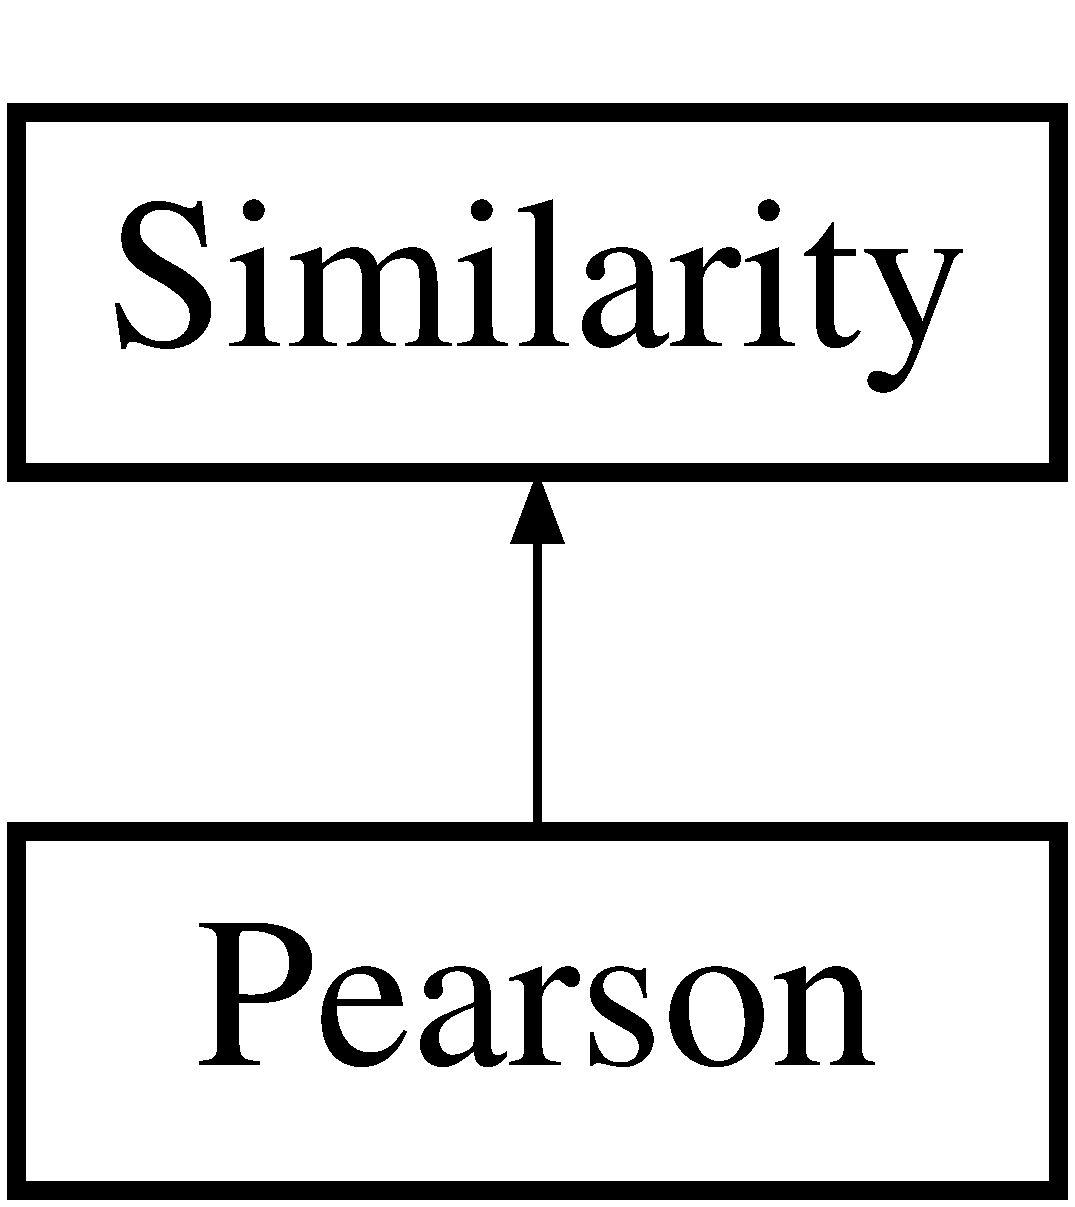
\includegraphics[height=2cm]{classPearson}
\end{center}
\end{figure}
\subsection*{Public Member Functions}
\begin{DoxyCompactItemize}
\item 
double \hyperlink{classPearson_a71d128fcaecda770e5b36494a916252f}{calculate} (const vector$<$ double $>$ \&vectorPattern\_\-1, const vector$<$ double $>$ \&vectorPattern\_\-2)
\end{DoxyCompactItemize}


\subsection{Detailed Description}
Responsible to calculate the pearson correlation coefficient. Responsible to calculate the pearson correlation coefficient, this is made in calculate method 

Definition at line 15 of file Pearson.h.

\subsection{Member Function Documentation}
\hypertarget{classPearson_a71d128fcaecda770e5b36494a916252f}{
\index{Pearson@{Pearson}!calculate@{calculate}}
\index{calculate@{calculate}!Pearson@{Pearson}}
\subsubsection[{calculate}]{\setlength{\rightskip}{0pt plus 5cm}double Pearson::calculate (const vector$<$ double $>$ \& {\em vectorPattern\_\-1}, \/  const vector$<$ double $>$ \& {\em vectorPattern\_\-2})\hspace{0.3cm}{\ttfamily  \mbox{[}virtual\mbox{]}}}}
\label{classPearson_a71d128fcaecda770e5b36494a916252f}
Calculate the pearson correlation coefficient. \begin{DoxyReturn}{Returns}
the pearson correlation coefficient 
\end{DoxyReturn}


Implements \hyperlink{classSimilarity_a3ff3d3622d8a45b15531bc143308b2ae}{Similarity}.

Definition at line 18 of file Pearson.cpp.

The documentation for this class was generated from the following files:\begin{DoxyCompactItemize}
\item 
Pearson.h\item 
Pearson.cpp\end{DoxyCompactItemize}

\hypertarget{classRelationSDN}{
\section{RelationSDN Class Reference}
\label{classRelationSDN}\index{RelationSDN@{RelationSDN}}
}


{\ttfamily \#include $<$RelationSDN.h$>$}\subsection*{Public Member Functions}
\begin{DoxyCompactItemize}
\item 
\hypertarget{classRelationSDN_abc9dd5e8a1441965db4fe7d964ad9296}{
{\bfseries RelationSDN} (\hyperlink{classSimilarityMatrix}{SimilarityMatrix} objASimilarityMatrix, \hyperlink{classNnList}{NnList} objANnList, \hyperlink{classSimilarity}{Similarity} $\ast$pAObjSimilarity)}
\label{classRelationSDN_abc9dd5e8a1441965db4fe7d964ad9296}

\item 
\hyperlink{classSimilarityMatrix}{SimilarityMatrix} \hyperlink{classRelationSDN_a52f3944e7966f4ea3684069fff04e1a3}{getSimilarityMatrix} ()
\item 
\hyperlink{classSimilarity}{Similarity} $\ast$ \hyperlink{classRelationSDN_a8db644a112eae5dd35c2ca0e47d36ce1}{getSimilarity} ()
\item 
\hyperlink{classNnList}{NnList} \hyperlink{classRelationSDN_a7d4ae265a19587306975a8cdac7bb115}{getNnList} ()
\item 
void \hyperlink{classRelationSDN_a3a8936efd1fd9ae0736a4a5e360b34e6}{setSimilarityMatrix} (map$<$ string, map$<$ string, double $>$ $>$ mapObjMap)
\item 
void \hyperlink{classRelationSDN_ad16b958a06717abf76ff5a96d008534c}{setSimilarity} (\hyperlink{classSimilarity}{Similarity} $\ast$pObjSimilarity)
\item 
void \hyperlink{classRelationSDN_a403418b3fb4ec2be68f91d8b47428885}{setNnList} (map$<$ string, map$<$ string, double $>$ $>$ mapObjMap)
\end{DoxyCompactItemize}


\subsection{Detailed Description}
\begin{DoxyAuthor}{Author}
Gustavo Rodrigues 
\end{DoxyAuthor}
\begin{DoxySince}{Since}
12/03/10 
\end{DoxySince}
\begin{DoxyVersion}{Version}
2.0 This class stores an object in which the similarity is generated from this similarity matrix and is created from the list of nearest neighbors. 
\end{DoxyVersion}


Definition at line 23 of file RelationSDN.h.

\subsection{Member Function Documentation}
\hypertarget{classRelationSDN_a7d4ae265a19587306975a8cdac7bb115}{
\index{RelationSDN@{RelationSDN}!getNnList@{getNnList}}
\index{getNnList@{getNnList}!RelationSDN@{RelationSDN}}
\subsubsection[{getNnList}]{\setlength{\rightskip}{0pt plus 5cm}{\bf NnList} RelationSDN::getNnList ()}}
\label{classRelationSDN_a7d4ae265a19587306975a8cdac7bb115}
Return nearest neighbor list 
\begin{DoxyParams}{Parameters}
\item[{\em Don't}]have \end{DoxyParams}
\begin{DoxyReturn}{Returns}
Object \hyperlink{classNnList}{NnList} 
\end{DoxyReturn}


Definition at line 33 of file RelationSDN.cpp.

Referenced by Connectivity::calculate().\hypertarget{classRelationSDN_a8db644a112eae5dd35c2ca0e47d36ce1}{
\index{RelationSDN@{RelationSDN}!getSimilarity@{getSimilarity}}
\index{getSimilarity@{getSimilarity}!RelationSDN@{RelationSDN}}
\subsubsection[{getSimilarity}]{\setlength{\rightskip}{0pt plus 5cm}{\bf Similarity} $\ast$ RelationSDN::getSimilarity ()}}
\label{classRelationSDN_a8db644a112eae5dd35c2ca0e47d36ce1}
Return pointer measure similarity 
\begin{DoxyParams}{Parameters}
\item[{\em Don't}]have \end{DoxyParams}
\begin{DoxyReturn}{Returns}
Pointer \hyperlink{classSimilarity}{Similarity} 
\end{DoxyReturn}


Definition at line 29 of file RelationSDN.cpp.

Referenced by Silhouette::calculate(), and Deviation::calculate().\hypertarget{classRelationSDN_a52f3944e7966f4ea3684069fff04e1a3}{
\index{RelationSDN@{RelationSDN}!getSimilarityMatrix@{getSimilarityMatrix}}
\index{getSimilarityMatrix@{getSimilarityMatrix}!RelationSDN@{RelationSDN}}
\subsubsection[{getSimilarityMatrix}]{\setlength{\rightskip}{0pt plus 5cm}{\bf SimilarityMatrix} RelationSDN::getSimilarityMatrix ()}}
\label{classRelationSDN_a52f3944e7966f4ea3684069fff04e1a3}
Return object similarity Matrix 
\begin{DoxyParams}{Parameters}
\item[{\em Don't}]have \end{DoxyParams}
\begin{DoxyReturn}{Returns}
\hyperlink{classSimilarity}{Similarity} Matrix 
\end{DoxyReturn}


Definition at line 24 of file RelationSDN.cpp.\hypertarget{classRelationSDN_a403418b3fb4ec2be68f91d8b47428885}{
\index{RelationSDN@{RelationSDN}!setNnList@{setNnList}}
\index{setNnList@{setNnList}!RelationSDN@{RelationSDN}}
\subsubsection[{setNnList}]{\setlength{\rightskip}{0pt plus 5cm}void RelationSDN::setNnList (map$<$ string, map$<$ string, double $>$ $>$ {\em mapObjMap})}}
\label{classRelationSDN_a403418b3fb4ec2be68f91d8b47428885}
Set nearest neighbor list 
\begin{DoxyParams}{Parameters}
\item[{\em Matrix}]map \end{DoxyParams}
\begin{DoxyReturn}{Returns}
Don't have 
\end{DoxyReturn}


Definition at line 45 of file RelationSDN.cpp.

References NnList::setNnList().

Referenced by DataSet::addNewRelationSDN().\hypertarget{classRelationSDN_ad16b958a06717abf76ff5a96d008534c}{
\index{RelationSDN@{RelationSDN}!setSimilarity@{setSimilarity}}
\index{setSimilarity@{setSimilarity}!RelationSDN@{RelationSDN}}
\subsubsection[{setSimilarity}]{\setlength{\rightskip}{0pt plus 5cm}void RelationSDN::setSimilarity ({\bf Similarity} $\ast$ {\em pObjSimilarity})}}
\label{classRelationSDN_ad16b958a06717abf76ff5a96d008534c}
Set measure similarity 
\begin{DoxyParams}{Parameters}
\item[{\em Pointer}]similarity \end{DoxyParams}
\begin{DoxyReturn}{Returns}
Don't have 
\end{DoxyReturn}


Definition at line 41 of file RelationSDN.cpp.

Referenced by DataSet::addNewRelationSDN().\hypertarget{classRelationSDN_a3a8936efd1fd9ae0736a4a5e360b34e6}{
\index{RelationSDN@{RelationSDN}!setSimilarityMatrix@{setSimilarityMatrix}}
\index{setSimilarityMatrix@{setSimilarityMatrix}!RelationSDN@{RelationSDN}}
\subsubsection[{setSimilarityMatrix}]{\setlength{\rightskip}{0pt plus 5cm}void RelationSDN::setSimilarityMatrix (map$<$ string, map$<$ string, double $>$ $>$ {\em mapObjMap})}}
\label{classRelationSDN_a3a8936efd1fd9ae0736a4a5e360b34e6}
Set object \hyperlink{classSimilarity}{Similarity} Matrix 
\begin{DoxyParams}{Parameters}
\item[{\em Matrix}]map \end{DoxyParams}
\begin{DoxyReturn}{Returns}
Don't have 
\end{DoxyReturn}


Definition at line 37 of file RelationSDN.cpp.

References SimilarityMatrix::setMatrix().

Referenced by DataSet::addNewRelationSDN().

The documentation for this class was generated from the following files:\begin{DoxyCompactItemize}
\item 
RelationSDN.h\item 
RelationSDN.cpp\end{DoxyCompactItemize}

\hypertarget{classSilhouette}{
\section{Silhouette Class Reference}
\label{classSilhouette}\index{Silhouette@{Silhouette}}
}


{\ttfamily \#include $<$Silhouette.h$>$}Inheritance diagram for Silhouette::\begin{figure}[H]
\begin{center}
\leavevmode
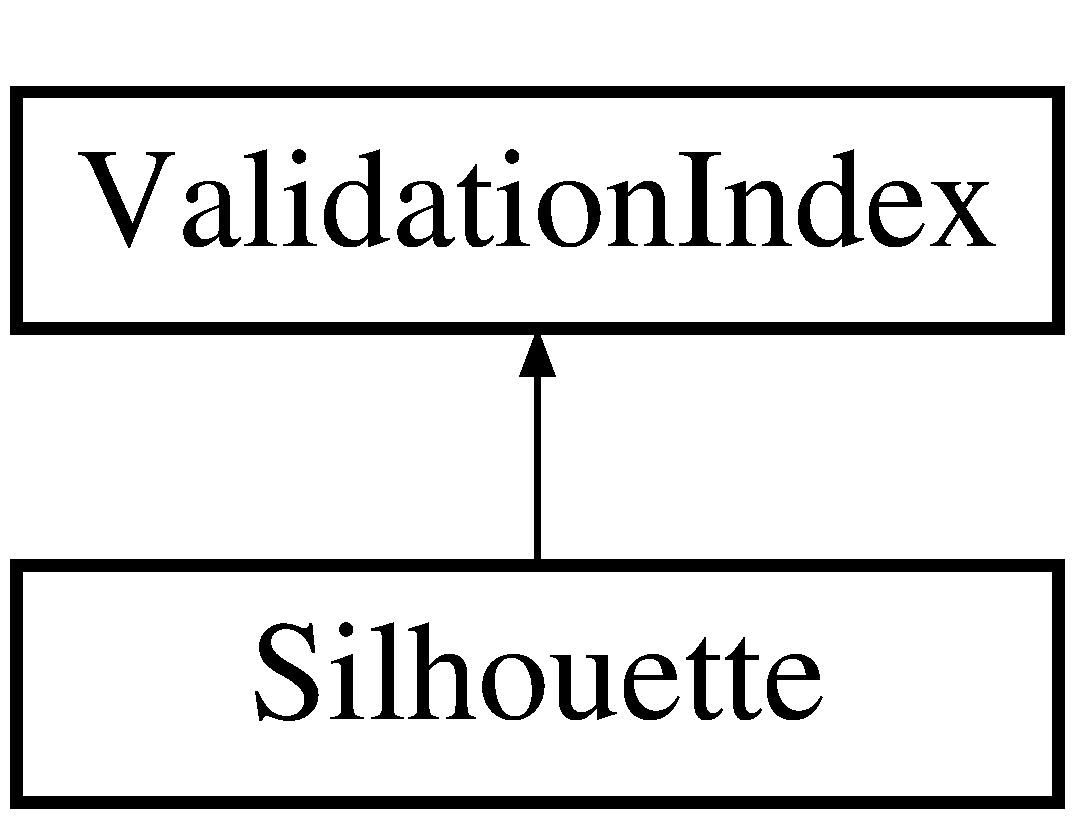
\includegraphics[height=2cm]{classSilhouette}
\end{center}
\end{figure}
\subsection*{Public Member Functions}
\begin{DoxyCompactItemize}
\item 
virtual double \hyperlink{classSilhouette_af8817c1accb7b60814cfff988c9ccc05}{calculate} (\hyperlink{classPartition}{Partition} $\ast$pAPartition, \hyperlink{classRelationSDN}{RelationSDN} $\ast$pARelation, \hyperlink{classDataSet}{DataSet} $\ast$pADataset)
\item 
virtual double \hyperlink{classSilhouette_aaf47b647b2409999209c58316ab8e980}{calculate} (\hyperlink{classPartition}{Partition} \&objPartition1, \hyperlink{classPartition}{Partition} \&objPartition2)
\end{DoxyCompactItemize}


\subsection{Detailed Description}
\begin{DoxyAuthor}{Author}
Gustavo Rodrigues 
\end{DoxyAuthor}
\begin{DoxySince}{Since}
22/03/10 
\end{DoxySince}
\begin{DoxyVersion}{Version}
2.0 
\end{DoxyVersion}


Definition at line 22 of file Silhouette.h.

\subsection{Member Function Documentation}
\hypertarget{classSilhouette_aaf47b647b2409999209c58316ab8e980}{
\index{Silhouette@{Silhouette}!calculate@{calculate}}
\index{calculate@{calculate}!Silhouette@{Silhouette}}
\subsubsection[{calculate}]{\setlength{\rightskip}{0pt plus 5cm}double Silhouette::calculate ({\bf Partition} \& {\em objPartition1}, \/  {\bf Partition} \& {\em objPartition2})\hspace{0.3cm}{\ttfamily  \mbox{[}virtual\mbox{]}}}}
\label{classSilhouette_aaf47b647b2409999209c58316ab8e980}
Does nothing 

Implements \hyperlink{classValidationIndex_a8b688d8d53fbdacec393730fe2bab614}{ValidationIndex}.

Definition at line 205 of file Silhouette.cpp.\hypertarget{classSilhouette_af8817c1accb7b60814cfff988c9ccc05}{
\index{Silhouette@{Silhouette}!calculate@{calculate}}
\index{calculate@{calculate}!Silhouette@{Silhouette}}
\subsubsection[{calculate}]{\setlength{\rightskip}{0pt plus 5cm}double Silhouette::calculate ({\bf Partition} $\ast$ {\em pAPartition}, \/  {\bf RelationSDN} $\ast$ {\em pARelation}, \/  {\bf DataSet} $\ast$ {\em pADataset})\hspace{0.3cm}{\ttfamily  \mbox{[}virtual\mbox{]}}}}
\label{classSilhouette_af8817c1accb7b60814cfff988c9ccc05}
Return value of silhouette from parameter partition 
\begin{DoxyParams}{Parameters}
\item[{\em \hyperlink{classPartition}{Partition},\hyperlink{classRelationSDN}{RelationSDN}}]and \hyperlink{classDataSet}{DataSet} \end{DoxyParams}
\begin{DoxyReturn}{Returns}
Value silhouette 
\end{DoxyReturn}


Implements \hyperlink{classValidationIndex_a26fe1244f3313bd7f557149f6846fe01}{ValidationIndex}.

Definition at line 18 of file Silhouette.cpp.

References Similarity::calculate(), DataSet::getMapVector(), Partition::getObjectsInCluster(), RelationSDN::getSimilarity(), and Partition::getVectorObjCluster().

The documentation for this class was generated from the following files:\begin{DoxyCompactItemize}
\item 
ValidationIndex/Silhouette.h\item 
ValidationIndex/Silhouette.cpp\end{DoxyCompactItemize}

\hypertarget{classSimilarity}{
\section{Similarity Class Reference}
\label{classSimilarity}\index{Similarity@{Similarity}}
}


Responsible by management the measures of similarity.  


{\ttfamily \#include $<$Similarity.h$>$}Inheritance diagram for Similarity::\begin{figure}[H]
\begin{center}
\leavevmode
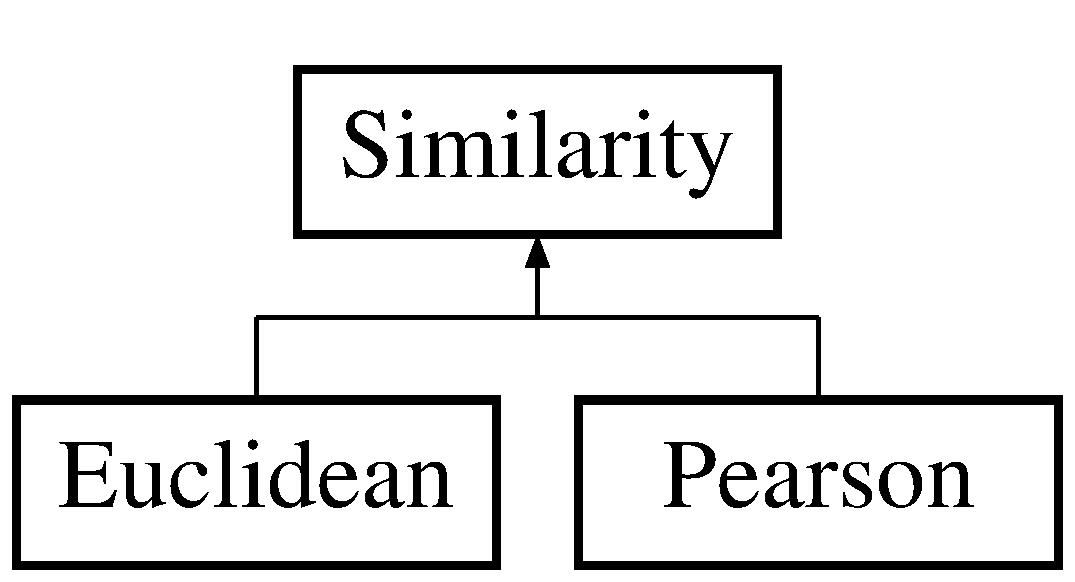
\includegraphics[height=2cm]{classSimilarity}
\end{center}
\end{figure}
\subsection*{Public Member Functions}
\begin{DoxyCompactItemize}
\item 
virtual double \hyperlink{classSimilarity_a3ff3d3622d8a45b15531bc143308b2ae}{calculate} (const vector$<$ double $>$ \&vectorPattern\_\-1, const vector$<$ double $>$ \&vectorPattern\_\-2)=0
\end{DoxyCompactItemize}


\subsection{Detailed Description}
Responsible by management the measures of similarity. \begin{DoxyAuthor}{Author}
Valter Henrique 
\end{DoxyAuthor}
\begin{DoxySince}{Since}
01/02/10 
\end{DoxySince}
\begin{DoxyVersion}{Version}
2.0 Responsible by management the measures of similarity, for example: Eucleadean Distance and Correlation \hyperlink{classPearson}{Pearson} 
\end{DoxyVersion}


Definition at line 25 of file Similarity.h.

\subsection{Member Function Documentation}
\hypertarget{classSimilarity_a3ff3d3622d8a45b15531bc143308b2ae}{
\index{Similarity@{Similarity}!calculate@{calculate}}
\index{calculate@{calculate}!Similarity@{Similarity}}
\subsubsection[{calculate}]{\setlength{\rightskip}{0pt plus 5cm}virtual double Similarity::calculate (const vector$<$ double $>$ \& {\em vectorPattern\_\-1}, \/  const vector$<$ double $>$ \& {\em vectorPattern\_\-2})\hspace{0.3cm}{\ttfamily  \mbox{[}pure virtual\mbox{]}}}}
\label{classSimilarity_a3ff3d3622d8a45b15531bc143308b2ae}
Each similarity class has the method 'calculate' that calculates the measures of similarity especific to that purpose 

Implemented in \hyperlink{classEuclidean_a732c1c959cc6978d4e9050bc42fda186}{Euclidean}, and \hyperlink{classPearson_a71d128fcaecda770e5b36494a916252f}{Pearson}.

Referenced by Silhouette::calculate(), Deviation::calculate(), and DataSet::generateMatrix().

The documentation for this class was generated from the following files:\begin{DoxyCompactItemize}
\item 
Similarity.h\item 
Similarity.cpp\end{DoxyCompactItemize}

\hypertarget{classSimilarityMatrix}{
\section{SimilarityMatrix Class Reference}
\label{classSimilarityMatrix}\index{SimilarityMatrix@{SimilarityMatrix}}
}


Generates the matrix of similarity.  


{\ttfamily \#include $<$SimilarityMatrix.h$>$}\subsection*{Public Member Functions}
\begin{DoxyCompactItemize}
\item 
map$<$ string, map$<$ string, double $>$ $>$ \hyperlink{classSimilarityMatrix_ad23f50845db414b67e3b37e5717c5633}{getMatrix} ()
\item 
void \hyperlink{classSimilarityMatrix_a5ee88b8eebc7987f7b5fd7ce04100b9d}{setMatrix} (map$<$ string, map$<$ string, double $>$ $>$ mapAObjMap)
\item 
\hypertarget{classSimilarityMatrix_a26e3f69ce969d1b164f22333b678d4b2}{
map$<$ string, map$<$ string, double $>$ $>$ {\bfseries getEuclideanMatrix} ()}
\label{classSimilarityMatrix_a26e3f69ce969d1b164f22333b678d4b2}

\item 
\hypertarget{classSimilarityMatrix_adcb0ca4d12e0c0468305927fd6e87c2e}{
map$<$ string, map$<$ string, double $>$ $>$ {\bfseries getPearsonMatrix} ()}
\label{classSimilarityMatrix_adcb0ca4d12e0c0468305927fd6e87c2e}

\item 
\hypertarget{classSimilarityMatrix_a1e1dbb2aa9575458a75e266180535286}{
void {\bfseries setEuclideanMatrix} (map$<$ string, map$<$ string, double $>$ $>$ mapAEuclidean)}
\label{classSimilarityMatrix_a1e1dbb2aa9575458a75e266180535286}

\item 
\hypertarget{classSimilarityMatrix_a9c7c6e31dc49a069d469dbd53cc98476}{
void {\bfseries setPearsonMatrix} (map$<$ string, map$<$ string, double $>$ $>$ mapAPearson)}
\label{classSimilarityMatrix_a9c7c6e31dc49a069d469dbd53cc98476}

\end{DoxyCompactItemize}


\subsection{Detailed Description}
Generates the matrix of similarity. \begin{DoxyAuthor}{Author}
Katti Facelli 
\end{DoxyAuthor}
\begin{DoxySince}{Since}
10/02/10 
\end{DoxySince}
\begin{DoxyVersion}{Version}
1.0 Generates the matrix of similarity 
\end{DoxyVersion}


Definition at line 30 of file SimilarityMatrix.h.

\subsection{Member Function Documentation}
\hypertarget{classSimilarityMatrix_ad23f50845db414b67e3b37e5717c5633}{
\index{SimilarityMatrix@{SimilarityMatrix}!getMatrix@{getMatrix}}
\index{getMatrix@{getMatrix}!SimilarityMatrix@{SimilarityMatrix}}
\subsubsection[{getMatrix}]{\setlength{\rightskip}{0pt plus 5cm}map$<$ string, map$<$ string, double $>$ $>$ SimilarityMatrix::getMatrix ()}}
\label{classSimilarityMatrix_ad23f50845db414b67e3b37e5717c5633}
Return the similarity matrix 
\begin{DoxyParams}{Parameters}
\item[{\em Don't}]have \end{DoxyParams}
\begin{DoxyReturn}{Returns}
\hyperlink{classSimilarity}{Similarity} matrix 
\end{DoxyReturn}


Definition at line 13 of file SimilarityMatrix.cpp.\hypertarget{classSimilarityMatrix_a5ee88b8eebc7987f7b5fd7ce04100b9d}{
\index{SimilarityMatrix@{SimilarityMatrix}!setMatrix@{setMatrix}}
\index{setMatrix@{setMatrix}!SimilarityMatrix@{SimilarityMatrix}}
\subsubsection[{setMatrix}]{\setlength{\rightskip}{0pt plus 5cm}void SimilarityMatrix::setMatrix (map$<$ string, map$<$ string, double $>$ $>$ {\em mapAObjMap})}}
\label{classSimilarityMatrix_a5ee88b8eebc7987f7b5fd7ce04100b9d}
Set similarity matrix 
\begin{DoxyParams}{Parameters}
\item[{\em Matrix}]map \end{DoxyParams}
\begin{DoxyReturn}{Returns}
Don't have 
\end{DoxyReturn}


Definition at line 16 of file SimilarityMatrix.cpp.

Referenced by RelationSDN::setSimilarityMatrix().

The documentation for this class was generated from the following files:\begin{DoxyCompactItemize}
\item 
SimilarityMatrix.h\item 
SimilarityMatrix.cpp\end{DoxyCompactItemize}

\hypertarget{classValidationIndex}{
\section{ValidationIndex Class Reference}
\label{classValidationIndex}\index{ValidationIndex@{ValidationIndex}}
}


{\ttfamily \#include $<$ValidationIndex.h$>$}Inheritance diagram for ValidationIndex::\begin{figure}[H]
\begin{center}
\leavevmode
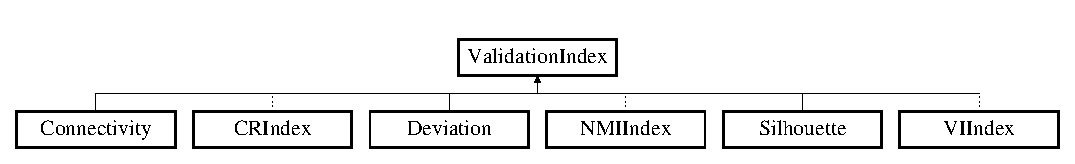
\includegraphics[height=1.76101cm]{classValidationIndex}
\end{center}
\end{figure}
\subsection*{Public Member Functions}
\begin{DoxyCompactItemize}
\item 
virtual double \hyperlink{classValidationIndex_a26fe1244f3313bd7f557149f6846fe01}{calculate} (\hyperlink{classPartition}{Partition} $\ast$pAPartition, \hyperlink{classRelationSDN}{RelationSDN} $\ast$pARelation, \hyperlink{classDataSet}{DataSet} $\ast$pDataSet)=0
\item 
virtual double \hyperlink{classValidationIndex_a8b688d8d53fbdacec393730fe2bab614}{calculate} (\hyperlink{classPartition}{Partition} \&objPartition1, \hyperlink{classPartition}{Partition} \&objPartition2)=0
\end{DoxyCompactItemize}


\subsection{Detailed Description}
Abstract class with two calculate methods, the one with two parameters is to be used in external validation measures and the one with one parameter is to be used in internal validation measures 

Definition at line 22 of file ValidationIndex.h.

\subsection{Member Function Documentation}
\hypertarget{classValidationIndex_a8b688d8d53fbdacec393730fe2bab614}{
\index{ValidationIndex@{ValidationIndex}!calculate@{calculate}}
\index{calculate@{calculate}!ValidationIndex@{ValidationIndex}}
\subsubsection[{calculate}]{\setlength{\rightskip}{0pt plus 5cm}virtual double ValidationIndex::calculate ({\bf Partition} \& {\em objPartition1}, \/  {\bf Partition} \& {\em objPartition2})\hspace{0.3cm}{\ttfamily  \mbox{[}pure virtual\mbox{]}}}}
\label{classValidationIndex_a8b688d8d53fbdacec393730fe2bab614}
Method virtual from return value of measure validation external 
\begin{DoxyParams}{Parameters}
\item[{\em \hyperlink{classPartition}{Partition}}]\end{DoxyParams}
\begin{DoxyReturn}{Returns}
Value from measure validation 
\end{DoxyReturn}


Implemented in \hyperlink{classConnectivity_a5f211e2c2ff7d5f199a985c6f6e68556}{Connectivity}, \hyperlink{classCRIndex_acfcf9186a522c78d67cc977aeddaf193}{CRIndex}, \hyperlink{classDeviation_af722cf601ea21cc689a77c1de470bcb5}{Deviation}, \hyperlink{classNMIIndex_a3d2c254720bd825119d1cd7905daa50f}{NMIIndex}, \hyperlink{classSilhouette_aaf47b647b2409999209c58316ab8e980}{Silhouette}, and \hyperlink{classVIIndex_ab097798a95465469bda061fbb57bf101}{VIIndex}.\hypertarget{classValidationIndex_a26fe1244f3313bd7f557149f6846fe01}{
\index{ValidationIndex@{ValidationIndex}!calculate@{calculate}}
\index{calculate@{calculate}!ValidationIndex@{ValidationIndex}}
\subsubsection[{calculate}]{\setlength{\rightskip}{0pt plus 5cm}virtual double ValidationIndex::calculate ({\bf Partition} $\ast$ {\em pAPartition}, \/  {\bf RelationSDN} $\ast$ {\em pARelation}, \/  {\bf DataSet} $\ast$ {\em pDataSet})\hspace{0.3cm}{\ttfamily  \mbox{[}pure virtual\mbox{]}}}}
\label{classValidationIndex_a26fe1244f3313bd7f557149f6846fe01}
Method virtual from return value of measure validation internal 
\begin{DoxyParams}{Parameters}
\item[{\em \hyperlink{classPartition}{Partition},\hyperlink{classRelationSDN}{RelationSDN}}]and \hyperlink{classDataSet}{DataSet} \end{DoxyParams}
\begin{DoxyReturn}{Returns}
Value from measure validation 
\end{DoxyReturn}


Implemented in \hyperlink{classConnectivity_ae132296aae336b3e3830431592611a74}{Connectivity}, \hyperlink{classCRIndex_a384b9fc6a5d271c13f7b599f17771041}{CRIndex}, \hyperlink{classDeviation_aefedb81474f0d06827a2ceaecd93f43c}{Deviation}, \hyperlink{classNMIIndex_a930fb32a05cbba0f427510536c204694}{NMIIndex}, \hyperlink{classSilhouette_af8817c1accb7b60814cfff988c9ccc05}{Silhouette}, and \hyperlink{classVIIndex_a0d43fc7805b4c05b97cea7c850216f5f}{VIIndex}.

The documentation for this class was generated from the following files:\begin{DoxyCompactItemize}
\item 
ValidationIndex.h\item 
ValidationIndex.cpp\end{DoxyCompactItemize}

\hypertarget{classVIIndex}{
\section{VIIndex Class Reference}
\label{classVIIndex}\index{VIIndex@{VIIndex}}
}


{\ttfamily \#include $<$VIIndex.h$>$}Inheritance diagram for VIIndex::\begin{figure}[H]
\begin{center}
\leavevmode
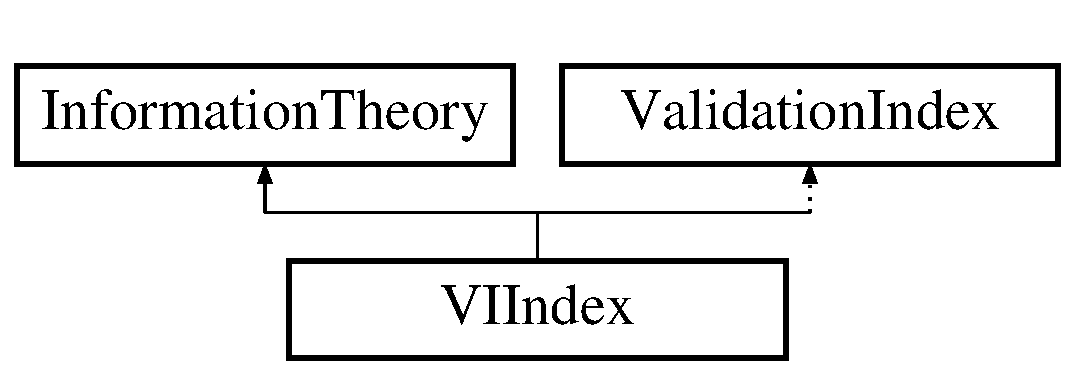
\includegraphics[height=2cm]{classVIIndex}
\end{center}
\end{figure}
\subsection*{Public Member Functions}
\begin{DoxyCompactItemize}
\item 
virtual double \hyperlink{classVIIndex_ab097798a95465469bda061fbb57bf101}{calculate} (\hyperlink{classPartition}{Partition} \&objPartition1, \hyperlink{classPartition}{Partition} \&objPartition2)
\item 
virtual double \hyperlink{classVIIndex_a0d43fc7805b4c05b97cea7c850216f5f}{calculate} (\hyperlink{classPartition}{Partition} $\ast$pPartition, \hyperlink{classRelationSDN}{RelationSDN} $\ast$pRelation, \hyperlink{classDataSet}{DataSet} $\ast$pDataset)
\end{DoxyCompactItemize}


\subsection{Detailed Description}
\begin{DoxyAuthor}{Author}
Vinicius 
\end{DoxyAuthor}
\begin{DoxySince}{Since}
??/$\backslash$?? 
\end{DoxySince}
\begin{DoxyVersion}{Version}
2.0 
\end{DoxyVersion}


Definition at line 17 of file VIIndex.h.

\subsection{Member Function Documentation}
\hypertarget{classVIIndex_a0d43fc7805b4c05b97cea7c850216f5f}{
\index{VIIndex@{VIIndex}!calculate@{calculate}}
\index{calculate@{calculate}!VIIndex@{VIIndex}}
\subsubsection[{calculate}]{\setlength{\rightskip}{0pt plus 5cm}double VIIndex::calculate ({\bf Partition} $\ast$ {\em pAPartition}, \/  {\bf RelationSDN} $\ast$ {\em pARelation}, \/  {\bf DataSet} $\ast$ {\em pDataSet})\hspace{0.3cm}{\ttfamily  \mbox{[}virtual\mbox{]}}}}
\label{classVIIndex_a0d43fc7805b4c05b97cea7c850216f5f}
Method virtual from return value of measure validation internal 
\begin{DoxyParams}{Parameters}
\item[{\em \hyperlink{classPartition}{Partition},\hyperlink{classRelationSDN}{RelationSDN}}]and \hyperlink{classDataSet}{DataSet} \end{DoxyParams}
\begin{DoxyReturn}{Returns}
Value from measure validation 
\end{DoxyReturn}


Implements \hyperlink{classValidationIndex_a26fe1244f3313bd7f557149f6846fe01}{ValidationIndex}.

Definition at line 15 of file VIIndex.cpp.\hypertarget{classVIIndex_ab097798a95465469bda061fbb57bf101}{
\index{VIIndex@{VIIndex}!calculate@{calculate}}
\index{calculate@{calculate}!VIIndex@{VIIndex}}
\subsubsection[{calculate}]{\setlength{\rightskip}{0pt plus 5cm}double VIIndex::calculate ({\bf Partition} \& {\em objPartition1}, \/  {\bf Partition} \& {\em objPartition2})\hspace{0.3cm}{\ttfamily  \mbox{[}virtual\mbox{]}}}}
\label{classVIIndex_ab097798a95465469bda061fbb57bf101}
Method virtual from return value of measure validation external 
\begin{DoxyParams}{Parameters}
\item[{\em \hyperlink{classPartition}{Partition}}]\end{DoxyParams}
\begin{DoxyReturn}{Returns}
Value from measure validation 
\end{DoxyReturn}


Implements \hyperlink{classValidationIndex_a8b688d8d53fbdacec393730fe2bab614}{ValidationIndex}.

Definition at line 8 of file VIIndex.cpp.

The documentation for this class was generated from the following files:\begin{DoxyCompactItemize}
\item 
ValidationIndex/VIIndex.h\item 
ValidationIndex/VIIndex.cpp\end{DoxyCompactItemize}

\printindex
\end{document}
